% Figures are pre-rendered PDFs; no EPS conversion is required.
\def\DoNotLoadEpstopdf{}
\documentclass[11pt,letterpaper]{article}

\usepackage[margin=1in]{geometry}
\usepackage[T1]{fontenc}
\usepackage[utf8]{inputenc}
\usepackage{lmodern}
\usepackage{microtype}
\usepackage{amsmath,amssymb}
\usepackage{booktabs,tabularx}
\usepackage{algorithm,algorithmic}
\usepackage{xcolor}
\usepackage{graphicx}
\usepackage[hidelinks]{hyperref}

\newcommand{\system}{Ferrule}
\renewcommand{\algorithmicrequire}{\textbf{Inputs:}}
\renewcommand{\algorithmicensure}{\textbf{Outputs:}}
\newcommand{\paperplot}[3]{%
  \begin{figure}[!htbp]
    \centering
    \includegraphics[width=\textwidth]{#1}
    \caption{#2}\label{#3}
  \end{figure}%
}

\title{Ferrule: Bounded Storage-Backed Weight Residency}
\author{Lu Huanbing\\Independent Researcher\\\texttt{luhuanbing084@gmail.com}}
\date{Working draft}

\begin{document}
\maketitle

\begin{abstract}
Storage-backed inference must bound temporary weight copies and prevent reuse
while reads, transfers, or device consumers still hold them. We present
\system{}, which connects source-bound materialization plans, stage-local
resource admission, and exact completion evidence to explicit ownership
through retirement. A bounded next-expert read schedule uses the same worker,
host and device budgets, and synchronous forward as a blocking control.
On Qwen3.5-35B-A3B, five paired blocks complete all 120 HTTP requests with
the prescribed output checks, identical logical reader work, zero wasted read bytes,
and logical host reservations below 64 MiB. In this configuration, the
prespecified paired summaries show 8.18\% lower end-to-end latency, 11.24\%
lower time to first content, and 10.91\% higher qualified serial-window
goodput with lookahead. Separate cache-budget, profiling, component-failure,
and HTTP-cancellation experiments clarify the mechanism's resource and
completion behavior. The five-block estimates are descriptive: shared
filesystem caches limit independence, logical budgets do not bound the
complete physical working set, and integrated fault conservation and final
physical release remain unverified.
\end{abstract}

\section{Introduction}
\label{sec:introduction}

Storage-backed inference repeatedly brings selected weights into an execution
cache rather than keeping every execution weight resident. This approach can
reduce device residency, but a small cache alone does not bound the resources
used to fill it. A read may retain host buffers, an upload may outlive its
caller, and an evicted binding may still have device consumers. Releasing a
logical request therefore does not necessarily make its capacity reusable.
The central problem is to coordinate weight materialization, resource admission,
and ownership through the last consumer.

Weight streaming and prefetch are established techniques in systems such as
FlexGen, ZeRO-Inference, and PowerInfer-2~\cite{sheng2023flexgen,deepspeed2022zeroinference,xue2024powerinfer2}.
Expert caches and speculative loading also address sparse demand in MoE
models~\cite{xue2024moeinfinity,eliseev2023fastmoeoffloading}.
SGLang also provides a specialized storage-backed expert path in the inspected
source~\cite{sglang2026expertpack}.
\system{} addresses a complementary architectural question: how should a
materialization schedule bind source identity, stage-local accounting, and
completion evidence so that capacity is not reused prematurely? We distinguish
three properties that are often conflated: a configured resource budget, a
measured physical working set, and evidence that a particular operation has
finished using its resources. Neither storage offload itself nor performance
leadership is the claimed novelty.

The design follows \emph{plan, admit, materialize, publish, execute, retire}.
A frozen plan identifies the source and destination generations. Admission
acquires the claims required by each stage. Completion validates the exact
operation before publication, while the owner retains buffers and charges
until the relevant consumers finish. If completion cannot be proved, the
intended discipline retains uncertain resources instead of treating an error
or cancellation as permission to reuse them. The resulting conservation model
is conditional on complete ownership and transfer rules; the serving evidence
observes selected host and expert-cache accounts, not every class in an
integrated system-wide ledger.

The implemented expert path separates read scheduling from transfer policy.
A persistent worker serves bounded checkpoint-read slots. The blocking schedule
waits at demand; lookahead submits one next-expert read before current expert
computation. Independently, grouped synchronous transfer batches the expert's
weight and scale copies behind one upload completion boundary. Both choices
preserve the expert order, arithmetic, and synchronous forward interface.
Worker lifetime, payload lifetime, upload completion, and device-consumer
retirement remain distinct: an idle live worker can still own charged metadata
and stack capacity.

\paragraph{Contributions.}
\begin{enumerate}
  \item An architecture for bounded storage-backed weight residency that connects
  source identity, stage-local admission, publication, and retirement, while
  distinguishing logical accounting from physical memory and producer completion
  from consumer quiescence.
  \item Reference algorithms for exact materialization and bounded cleanup,
  together with an implemented persistent read worker, bounded next-expert
  scheduling, and grouped synchronous expert uploads.
  \item A profile-scoped evaluation linking numerical and HTTP output checks,
  logical work and resource accounts, client timing, selected-process profiling,
  and component-failure and cancellation behavior, including negative results.
\end{enumerate}

\paragraph{Research questions.}
\begin{description}
  \item[RQ1: Bounded completion.] Can requests complete under the declared
  accounting policies, and how does residency change across coupled cache budgets?
  \item[RQ2: I/O demand.] What work reaches the logical reader and shared
  filesystem client, and which physical traffic remains unknown?
  \item[RQ3: Scheduling and transfer.] How do read scheduling and upload grouping
  affect observed waiting, synchronization, and client outcomes?
  \item[RQ4: Failure and custody.] What resources and state remain after
  clean abort, uncertain completion, and HTTP cancellation?
\end{description}

The core serving workload uses Qwen3.5-35B-A3B-FP8 through the public CLI,
with BF16 execution weights and explicitly defined F32 boundaries, not a
full-model W8A16 quality claim. Four acceptance servers complete 48 checked
requests. A separate grouped-versus-synchronous transfer pilot completes eight
fresh server lifecycles and 96 requests, including 40 measured eight-token
quality checks. With lookahead, grouped uploads reduce observed client latency
and increase phase-qualified goodput; with blocking reads, time to first content
regresses despite nearly unchanged end-to-end latency. There are only two
pairs per read schedule. An earlier five-pair read-scheduling study instead
compares blocking with lookahead under its own fixed implementation, finding
less demand waiting and lower observed client latency with equal logical reads.
These are separate comparisons, not a pooled population or evidence of a
universal improvement.

The evaluation establishes neither a physical capacity frontier nor a matched
external-system ranking. DeepSeek-V4 end-to-end execution is untested;
architecture-level applicability does not qualify another model adapter.
Table~\ref{tab:evidence} consolidates the measurement boundaries.
Section~\ref{sec:scope} defines the model and assumptions.
Section~\ref{sec:design} develops the mechanisms and algorithms, and
Section~\ref{sec:implementation} maps them to the implemented path.
Section~\ref{sec:eval-setup} fixes the methodology before
Section~\ref{sec:evaluation} answers the four questions. Related work,
limitations, and separate historical evidence follow.

\section{Resource Model and Execution Contracts}
\label{sec:scope}

\subsection{Representations and one notation}
The target is a complete request or forward output under a declared model,
arithmetic, placement, and quality profile $\pi$. Text decoding is the current
instance: prefill, multiple decode steps, and KV/state lifetime. Vision,
audio, and combined modalities require their own complete-output contracts
and remain future implementation and evaluation work.

A representation $r$ identifies payload, decoding metadata, expansion, and
required physical copies. Checkpoint bytes $S_{\mathrm{ckpt}}$ include the
specified files and container layout. Complete compact weights
$W_{\mathrm{compact}}$ include all encoded weights, scales, and decoding
metadata. Full-resident weight demand $W_{\mathrm{full}}(r)$ is the footprint
of all weights under representation and placement $r$; it is weight-only,
not the complete inference working set. Expanded execution weights may be
larger than compact weights and need not all be live at once. Aliased views
are not extra copies; genuinely copied payloads are.

\begin{table}[tbp]
\centering
\small
\begin{tabularx}{\linewidth}{@{}l>{\raggedright\arraybackslash}X@{}}
\toprule
Symbol & Meaning and units \\
\midrule
$\pi,r$ & Execution/quality profile and weight representation/placement \\
$S_{\mathrm{ckpt}},W_{\mathrm{compact}},W_{\mathrm{full}}(r)$ & Checkpoint, complete compact, and full-resident weight bytes \\
$d\in\mathcal D_{\mathrm{phys}},B_d$ & Disjoint physical domain and available physical byte capacity \\
$a\in\mathcal D_{\mathrm{acct}},b_a$ & Covered accounting domain and configured limit in that domain's unit \\
$M_d(t),M_d^{\mathrm{peak}}$ & Deduplicated physical working-set bytes at time $t$, and its true peak \\
$\widehat M_d(t_i),\widehat M_d^{\mathrm{max}}$ & Reported sample and maximum over stated sampling times; not a true peak \\
$U_a(t),c_a$ & Charged occupancy and additional proposed claim, in domain $a$'s unit \\
$\delta,\rho_a,b_a^{\mathrm{eff}}(\delta)$ & Demand class, execution reserve, and its policy-accessible accounting ceiling \\
$F_a,R_a,I_a,L_a,T_a$ & Free, reserved, provider-in-flight, live, and retained claims \\
$P=(K,\boldsymbol q,\boldsymbol\ell)$ & Frozen plan: exact key, stage claim vectors, resident claim vector \\
$K,g_s,g_x$ & Full resource key, source generation, destination reuse generation \\
$o,e,J$ & Owned operation, completion evidence, provisional owner journal \\
$\Omega,k,w,\mu_o[s]$ & Post-detachment worklist, per-pass visit limit, persistent cursor, and exact-stage cancellation marker \\
$\mathcal V_q,L_q,H_q,\Delta_q$ & Request $q$'s invocations, logical reader bytes, facade H2D bytes, and $H_q-L_q$ \\
$N_j,I_j,E_j$ & Expert entries at invocation boundary $j$, installs/uploads, and evictions \\
$X_j,Q_j,S_j,C_j^{\mathrm{cache}},Z_j$ & Resident, pending-upload, scratch, cache charge, and retained Unknown subset gauges \\
$C_{\mathrm{peak}}^{\mathrm{cache}}$ & Lifetime cache-accounting high-water; not a total physical-owner peak \\
$P_q^{\mathrm{net}},P_q^{\mathrm{blk}}$ & Physical network and backing-block bytes attributed to request $q$ \\
$b_{\mathrm{cache}},b_{\mathrm{scratch}}$ & Configured cache-credit and scratch limits; neither is a physical-domain bound \\
\bottomrule
\end{tabularx}
\caption{Notation used by the contracts, algorithms, and evaluation.
Accounting limits are never substituted for physical capacity.}
\label{tab:symbols}
\end{table}

\subsection{Physical capacity and measured working set}
Physical capacity counts disjoint resident-memory pools once:
\begin{equation}
 B_{\mathrm{mem}}=\sum_{d\in\mathcal D_{\mathrm{phys}}}B_d.
 \label{eq:physical-capacity}
\end{equation}
For a declared representation and placement, consider
\begin{equation}
 W_{\mathrm{full}}(r)>B_{\mathrm{mem}}.
 \label{eq:full-residency}
\end{equation}
The inequality rules out aggregate full residency of \emph{that}
representation/placement, not streaming feasibility. Disk is excluded.
Discrete host and GPU pools may be added; host and accelerator aliases of
one physical pool may not. Unified virtual addressing over separate physical
pools does not merge those pools. Report installed capacity, fixed exclusions,
co-tenants, copies, and placement/migration policy for each evaluated domain.
Per-domain accessibility and placement remain constraints even when the
aggregate sum is sufficient.

Define $M_d(t)$ as physical bytes resident in domain $d$ that are attributable
to the selected inference deployment at time $t$. Count resident weights,
expansion/workspace, activations, model state, staging, outstanding and retained
buffers, metadata, allocator/driver reserves, and attributable file-backed
pages, deduplicating shared physical allocations. A full attribution requires
fixed and external consumers to be measured or excluded explicitly; a
process heap or device counter alone does not supply it. The desired
feasibility condition and the reported sampling statistic are different:
\begin{equation}
\begin{aligned}
 M_d^{\mathrm{peak}}&=\sup_{t\in\mathcal T}M_d(t)\leq B_d
       &&\text{for each }d,\\
 \widehat M_d^{\mathrm{max}}&=\max_{t_i\in\mathcal T}
       \widehat M_d(t_i)
       &&\text{over the declared samples.}
\end{aligned}
\label{eq:working-set}
\end{equation}
$\mathcal T$ is the declared startup/request/cleanup interval. A sampled
maximum can miss a transient peak; selected-device telemetry also includes
unattributed processes, and tree PSS does not cover every machine consumer.
Thus those proxies are not silently identified with $M_d(t)$. Independent
component maxima must not be added into a simultaneous working-set peak.
RQ1 uses Table~\ref{tab:tp1-memory}; the storage-demand figures in
Section~\ref{sec:rq2} diagnose cache and transfer counters without turning
sample maxima into certified physical bounds.

The storage-necessity gate additionally asks whether \emph{all compact
weights and metadata} can remain resident with online expansion under the
quality contract. Failure to fit expanded weights is insufficient if that
compact alternative fits. A low configured cache budget is likewise not
physical host-memory insufficiency. Storage necessity is scoped to evaluated
representations, not a proof against every possible compression scheme.

\subsection{Accounting and admission contract}
A covered accounting domain $a$ may count bytes, slots, pages, or queue entries.
Its limit $b_a$ is configured, not installed physical capacity; accounting
domains can overlap or omit parts of a pool and cannot in general be summed.
A cache limit covers its cache, not the whole working set. The necessary
covered-domain capacity condition is
\begin{equation}
 \forall a\in\mathcal D_{\mathrm{acct}},\qquad
 U_a(t)+c_a\leq b_a.
 \label{eq:admission}
\end{equation}
Here $c_a$ is the additional charge to acquire, not a second charge for an
already held grant. A revisit preserves that grant and rechecks only unmet
claims. The inequality is not sufficient for admission: the owner must also
validate canonical claims and units, arithmetic overflow,
source/placement/backend compatibility,
actual reservation and grant authority, and the selected demand policy.
With execution reserve $0\leq\rho_a\leq b_a$, the policy-accessible ceiling is
\begin{equation}
 b_a^{\mathrm{eff}}(\delta)=
 \begin{cases}
 b_a,&\delta=\mathsf{Required},\\
 b_a-\rho_a,&\delta\in\{\mathsf{Warmup},\mathsf{Prefetch}\}.
 \end{cases}
 \label{eq:execution-reserve}
\end{equation}
A non-required demand cannot consume the execution reserve even if
Equation~\ref{eq:admission} holds. Required execution may use that reserve,
not exceed the hard ceiling. The reserve protects accounting capacity from
speculation, not eventual progress against a stalled provider.

The abstract admission result has three cases. \textsf{Rejected} includes
invalid plans and an intrinsically impossible stage: for example, a required
claim exceeding $b_a$, or a non-required claim exceeding its unchanged
policy-accessible ceiling even with no other occupancy. Waiting cannot fix
such a stage; it needs rejection or an explicitly changed, revalidated plan
or demand policy. \textsf{Wait} means the otherwise admissible stage is
blocked by current occupancy, including reserve-protected capacity. It retains
existing claims and registers a revisit condition rather than recharging or
redispatching them. \textsf{Admitted} requires all authority, compatibility,
and policy checks as well as capacity. These are explanatory result classes,
not a new backend API, and do not imply that all future stages can be admitted
atomically or that their resource waits are acyclic.

Each claim has an authoritative owner, unit, and end condition. Canonicalizing
same-kind claims is not deduplication of arbitrary aliased allocations. A
bounded request channel does not bound all downstream buffers. Map claims to
the actual ledger and physical allocations on the selected path; do not infer
one global broker from a common interface.

The plan $P$ binds $K$, read/upload/install claim vectors $\boldsymbol q$,
and persistent residency $\boldsymbol\ell$. $K$ includes model instance,
source identity, semantic content descriptor, encoding, backend/device,
and $g_s,g_x$. Alignment and multiple extents may change staged byte counts;
expansion may change execution bytes. The destination authority supplies the
actual reservation and $g_x$ before hard admission. Publication consumes
validated bindings, not requested addresses. Algorithm~\ref{alg:normal-materialization}
uses the capacity and policy checks in Equations~\ref{eq:admission}
and~\ref{eq:execution-reserve} before each physical dispatch.

OS page cache, storage-server cache, metadata, and driver reserves are not
implicitly under runtime credit control. Resident file-backed pages count as
memory; the backing file adds no capacity. Swap must be disabled or explicitly
accounted for. A logical read, page fault, or migration between physical pools
is not evidence of a physical storage read. RQ2 consequently distinguishes
$L_q,H_q,\Delta_q,P_q^{\mathrm{net}},P_q^{\mathrm{blk}}$ rather than translating
them into one bandwidth number.

\subsection{Quality, completion, and progress contracts}
Protocol exactness means compatible sharing, exact completion identity,
authorized publication, and no reuse before physical references end. It is
separate from numerical/task quality. A quality contract fixes complete
outputs, independent reference, arithmetic/state precision, inputs, and
acceptance thresholds. Visible text, usage, generated IDs, full-vocabulary
logits, ordered routes, and internal states are different checks; argmax
agreement does not establish numerical agreement. Quantized checkpoint
storage alone does not specify kernel or KV arithmetic.

Completion evidence must name its operation, full key, submitted stage,
generations, outcome-specific byte count, and any required physical fence.
Rejecting an event with mismatched identity, stage, generation, or byte
contract is not the same as accepting a matching event whose validated
\texttt{CompletionOutcome::Stale} is a non-success result. The former supplies
no mutation/release authority; the latter selects terminal cleanup of its
named operation, never readiness or publication of a newer generation.
Returning named read custody is separate from releasing the read-slot and
storage-read claims; pinned host capacity remains charged through upload or
proven cleanup. Publication preflight similarly distinguishes Ready, Blocked
by live replacement custody, and Rejected by an invalid binding/conflict.
Rejected publication retains its journal and remaining custody for cleanup.

Only validated producer success proves readiness of that stage, not
quiescence of a later consumer. Only owner-accepted cancellation selects a
canceled caller outcome and detaches demand; a cancellation request or provider acceptance
alone does not prove physical completion. Shared loads retain their remaining
owners. Pending/Idle is retained as Pending only for a positively known
original pollable obligation; otherwise it retains Unknown custody. Unknown
means remaining physical references cannot be proved. Unknown retains allocation
and credits, possibly indefinitely. A late exact scoped completion can close
its named registry obligation but cannot clear physical-owner poison or
quarantine. Bounded cleanup passes retain unresolved obligations and a
traversal cursor across wakes and revisits, so the same first items do not hide unvisited
obligations. Ambiguous cancellation replies remain non-retryable without
exact owner evidence; they are not treated as known non-acceptance. Neither
that scheduling contract nor Unknown retention promises eventual reclamation
or availability.

Conditional liveness requires feasible per-domain resources, no cyclic
resource waits, fair progress and completion handling, live providers, and
eventually observable completion. A blocking provider or stalled progress
worker can violate these conditions. An asynchronous API, event-driven
progress, and hardware overlap are separate properties. Neither algorithms
nor current receipts establish global nonblocking execution, lock freedom,
durable crash recovery, or arbitrary multi-owner atomic commit.

\section{A Normal Profile Walkthrough}
\label{sec:design}
\label{sec:normal-profile}

Consider a profile $\pi$ with a nonresident weight dependency. The following
walkthrough composes protocol roles; it is not a claim that every TP1 runner
uses the general registry. It connects the resource model to the algorithms
and to the observables evaluated in Section~\ref{sec:evaluation}.

\paragraph{Plan and admit.}
The adapter binds source descriptors, representation, placement, and workspace.
The destination authority supplies the actual reservation and reuse generation.
The resulting $P=(K,\boldsymbol q,\boldsymbol\ell)$ is frozen before hard
admission. Equation~\ref{eq:admission} is a necessary covered-domain check,
not complete admission or a sum of heterogeneous budgets. The stage also
passes authority, compatibility, intrinsic-capacity, and execution-reserve
checks in Section~\ref{sec:scope}. An impossible stage is rejected; only
otherwise admissible demand blocked by current occupancy waits. Before preparation can submit physical
work, the owner records provisional state and cleanup intent in journal $J$.

\paragraph{Read, transfer, and install.}
A new load admits read/staging claims and submits once. Exact read completion
returns named read custody. On read success, the owner then explicitly
releases held ReadSlot and StorageReadBytes credits while retaining the
pinned buffer and PinnedHostBytes charge for upload. Custody return alone
is not that credit discharge. Upload needs
its own admission and retained fence; its completion ends DMA custody but not
destination ownership. Installation admits its own claims. Replacement also
needs evidence that old consumers have stopped using the old binding. An
ambiguous submission retains its ticket, allocations, and claims even when no
public handle is returned.

\paragraph{Publish and consume.}
Install success is validated against operation, key, stage, bytes, and both
generations. Publication preflight checks the actual binding and replacement
rules. Ready permits resident-grant transfer and exact waiter resolution;
Blocked waits for replacement leases/custody to end; Rejected preserves the
original journal, grants, and physical binding for terminal cleanup instead
of publishing or refunding residency. Only Ready retires the load operation
by transferring its resident grant. This is not eviction: resident bytes
remain charged. A consumer revalidates its dependency and lease epochs and
obtains resume admission before executing. A compatible resident hit skips
materialization; a compatible in-flight load can be joined only on paths that
implement sharing.

\paragraph{Bounded next-expert scheduling.}
On the concrete routed-expert path, the owner first uploads the current
expert and retires its temporary host payload aliases. It can then submit one
read for the next selected, nonresident expert before submitting current
compute. A read-only residency hint neither pins that next expert nor changes
cache replacement order. Blocking uses the same worker and waits at demand
instead. This split is a scheduling candidate, not a measured GPU overlap or
an asynchronous forward API (Algorithm~\ref{alg:bounded-lookahead}).

\paragraph{End and retire.}
Consumer completion returns only the custody discharged by its adapter.
Ending/publication and post-ending cleanup are separate phases. Prepared-KV
owners require exact install acknowledgments before logical publication and
retirement acknowledgments before displaced pages are reused. Independent
cache pins and persistent state survive request completion. Cancellation
changes the caller outcome, not these end conditions; Unknown may retain
capacity indefinitely.

\begin{figure}[tbp]
\centering
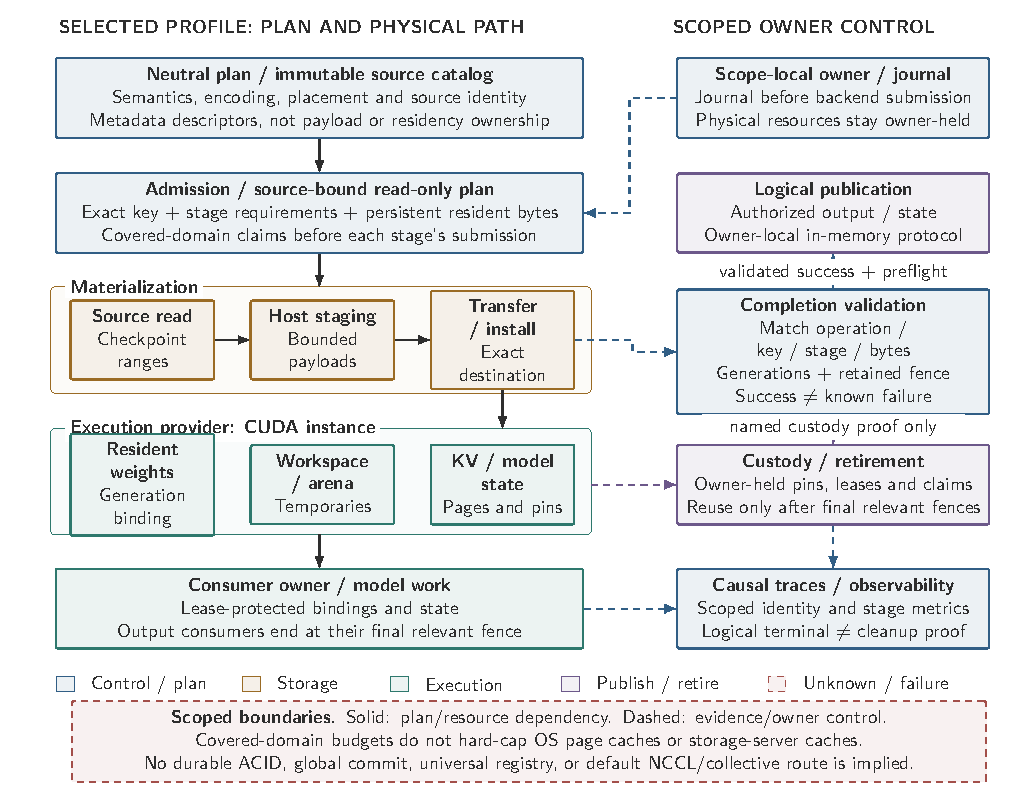
\includegraphics[width=\linewidth]{figures/architecture.pdf}
\caption{Conceptual, profile-scoped architecture. The shared palette uses blue
for control/planning/validation, ochre for storage/materialization, teal for
execution/provider resources, violet for publication/custody/retirement, and
brick for Unknown/failure. Named nodes and labeled swatches carry the meaning
independently of color. Solid arrows denote dependencies; dashed arrows name
evidence or owner-control gates. Source planning and covered-domain admission
precede materialization; providers retain physical resources. CUDA is one
provider instance. No universal registry, OS-cache hard cap, durable/cross-rank
ACID, or default NCCL/device-collective route is implied.}
\label{fig:architecture}
\end{figure}

The walkthrough supplies three different evidence gates: startup final-claim
completion, materialization producer/replacement completion, and consumer/
ending completion. None substitutes for another. The experiment should record
those transitions alongside complete-output quality, physical memory samples,
and request I/O. The arrows in Figure~\ref{fig:architecture} are conceptual
dependencies, not measured hardware overlap.

\section{Design Invariants}
\label{sec:invariants}

These are intended contracts for the implemented boundaries, not completed
formal verification or independently measured properties of every profile.

\paragraph{I1: bounded, uniquely owned claims.}
Admitted claims must preserve $U_a+c_a\leq b_a$, together with the demand
policy and authority checks; this inequality alone is not admission. For each accounting domain, the
intended semantic partition is
\begin{equation}
\begin{aligned}
 b_a&=F_a+R_a+I_a+L_a+T_a,\\
 U_a&=R_a+I_a+L_a+T_a,\qquad F_a=b_a-U_a .
\end{aligned}
\label{eq:credit-conservation}
\end{equation}
Each claim occupies exactly one class: free, reserved, provider-in-flight,
live, or retained. Different claims of one operation can occupy different
classes. Unknown is classified in $T_a$, not charged again as $I_a+T_a$.
Returning provider custody does not necessarily decrease $U_a$: an explicit
release or ownership transfer is separate. The broker records capacity,
occupancy, authenticated owner, and a submitted bit, not five literal bucket
fields. Equation~\ref{eq:credit-conservation} is an intended invariant;
the serving read ledger does not independently measure this general partition
under faults. RQ4 separates observed owner-local closure from the missing
integrated fault and physical-release evidence.

\paragraph{I2: exact evidence before mutation.}
A completion must match $o$, $K$, submitted stage, $g_s$, $g_x$, and
outcome-specific bytes. Success requires the full expected amount; partial
failure is not readiness. Identity-stale, retired, unowned, wrong-stage,
or generation-mismatched events are rejected before mutation and cannot
release a newer generation's grants. In contrast, a matching completion whose
validated \texttt{CompletionOutcome::Stale} reports non-success ends the
named stage according to its proof and selects terminal cleanup; it is not
an identity rejection and does not authorize publication.
Waiter/request/dependency epochs and mapping epochs have different scopes;
a wake notification is not validation of any of them.

\paragraph{I3: custody follows physical work.}
Every outstanding physical reference is required to remain reachable from an
authoritative owner, including on submission, notification, preparation, or cleanup errors.
Read return, upload-fence return, resident transfer, and consumer retirement
close different obligations. An address descriptor is not allocation ownership
or a completion certificate. A read snapshot is not mutation authority.

\paragraph{I4: publication and reuse have different proofs.}
Producer success makes a candidate ready. Publication additionally checks the
actual binding and authorization; old-consumer quiescence and retirement
permit replacement reuse. Typed committed-KV sources and append witnesses are
revalidated against the current page authority, and zero-reference pages are
reused only after retirement confirmation. Several participant ACKs establish
this scoped lifecycle order, not arbitrary distributed atomic commit.

\paragraph{I5: terminal demand does not erase obligations.}
Owner-accepted cancellation detaches only its demand, preserving other
waiters and persistent owners. An unsubmitted shared load is preserved under
its remaining authority or handed off with acknowledgment, never discarded
because one demand ended. Provider cancellation acceptance is recorded once
per exact operation/stage/generation; it is not a quiescence certificate. It cannot reverse an irreversible install/publish intent. Pending
cleanup polls the original identity and arguments without redispatch. Unknown
retains physical payload and credits and preserves applicable owner poison or
quarantine. A matching later registry completion may close a named stage; it
cannot heal a separately poisoned physical owner. No general in-place reset/
replay or unconditional eventual reclamation is asserted.

\begin{figure}[tbp]
\centering
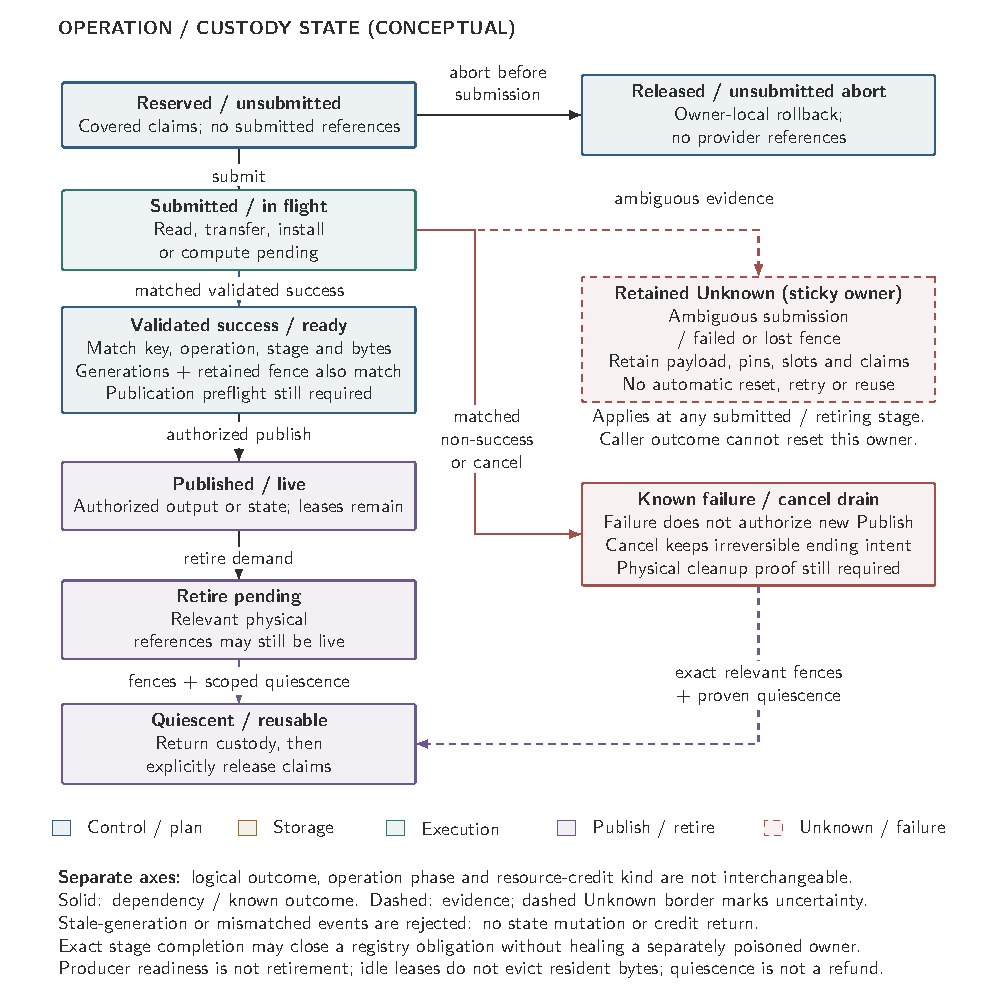
\includegraphics[width=\linewidth]{figures/operation-state.pdf}
\caption{Conceptual operation/custody states, not one Rust enum. Labeled roles
retain the shared blue planning/validation, ochre storage, teal execution,
violet publication/retirement, and brick Unknown/failure palette. Only exact
validated success plus publication preflight authorize new publication.
Known non-success drains the named stage, not readiness; cancellation keeps
irreversible ending intent. Dashed-border physical-owner Unknown retains
payload, pins, slots, and claims and has no automatic recovery/reuse edge.
Closing a matching registry-stage obligation does not heal a separately
poisoned owner. Logical outcomes and charged resources are separate axes.}
\label{fig:operation-state}
\end{figure}

The testable consequences are no stale publication, no duplicate dispatch,
no premature slab/page reuse, and retained capacity when proof is missing.
RQ1 checks bounded completion, RQ2 checks the load demand, RQ3 checks progress
and physical intervals, and RQ4 checks these invariants under faults. A process
exit or idle sample does not independently prove any final owner ledger.

\section{Lifecycle and Bounded Scheduling Algorithms}
\label{sec:algorithms}

The pseudocode names protocol roles and abstract result classes, not new
provider APIs. Its records and journal persist across calls. \textsc{AdmitStage}
validates intrinsic feasibility, canonical claims, authority, compatibility,
and demand/reserve policy before acquiring that stage's grants. An added
claim $c_a>b_a^{\mathrm{eff}}(\delta)$ is intrinsically impossible under that
policy; an otherwise feasible claim blocked by current
$U_a+c_a>b_a^{\mathrm{eff}}(\delta)$ waits. The authoritative owner rechecks
capacity on acquisition, without implying a cross-owner atomic reservation. Rejected
means no further dispatch under the unchanged plan; Wait preserves already
held custody and arms a budget/owner-progress revisit. \textsc{RetainCleanup}
records the primary reason and original payload, then selects the cleanup
protocol in Algorithm~\ref{alg:terminal-custody}; it does not recreate a ticket
or discard other demand. Publication Rejected is the abstract class for
preflight validation/conflict errors, distinct from a live-custody Blocked
result. Rejection after install does not undo the physical installation.
The owner journal records applied custody returns and releases so later
cleanup advances only residual obligations, without applying a return twice.
Cleanup selection is latched: subsequent calls cannot restart normal dispatch
or replace the primary failure reason. Pending/Idle requires a positively
known original pollable obligation; otherwise its custody is Unknown and
retained. Unknown follows cleanup without clearing physical-owner poison.

\begin{algorithm}[tbp]
\caption{Progress one exact materialization operation}
\label{alg:normal-materialization}
\fontsize{9}{9.4}\selectfont
\begin{algorithmic}[1]
\REQUIRE $P:\mathsf{Plan}$, $v:\mathsf{Provider}$, $\mathcal L:\mathsf{Ledger}$,
         $\delta:\mathsf{Demand}$, $J:\mathsf{Journal}$
\ENSURE $h:\{\mathsf{Ready},\mathsf{Pending},\mathsf{Terminal}\}$, $o:\mathsf{LoadRecord}$; residual custody stays reachable
\STATE \textbf{State:} persistent $o:\mathsf{LoadRecord}$; $s:\mathsf{Stage}$;
       $e:\mathsf{Evidence}$; $p:\mathsf{PublicationResult}$;
       $\alpha:\mathsf{AdmissionResult}$
\STATE \textbf{Preconditions:} frozen plan, exact destination, authoritative
       journal; residency/sharing checked
\IF{cleanup is selected or $o$ has retained Unknown}
  \STATE preserve $J,o$; continue only Algorithm~\ref{alg:terminal-custody}
  \RETURN $(\mathsf{Terminal},o)$
\ENDIF
\WHILE{$o.\mathit{phase}\ne\mathsf{Resident}$}
  \IF{$o.\mathit{phase}=\mathsf{Installed}$}
    \STATE \textbf{Publication:} $p\gets\operatorname{Preflight}(o)$
    \IF{$p=\mathsf{Ready}$}
      \STATE publish exact binding; transfer resident grant
      \STATE resolve exact waiters; retire once; $o.\mathit{phase}\gets\mathsf{Resident}$
    \ELSIF{$p=\mathsf{Blocked}$}
      \STATE retain $J,o$; arm replacement-custody revisit
      \RETURN $(\mathsf{Pending},o)$
    \ELSIF{$p=\mathsf{Rejected}$}
      \STATE $\operatorname{RetainCleanup}(J,o,p)$; \algorithmicreturn $(\mathsf{Terminal},o)$
    \ENDIF
  \ELSE
    \STATE $s\gets o.\mathit{stage}$
    \IF{stage $s$ is not submitted}
      \STATE \textbf{Admission:} validate/canonicalize units, overflow, authority,
      \STATE source/placement/backend compatibility, and demand policy
      \IF{validation fails or $\exists a: c_a>b_a^{\mathrm{eff}}(\delta)$}
        \STATE $\alpha\gets\mathsf{Rejected}$ with invalid-plan/intrinsic-capacity reason
        \STATE $\operatorname{RetainCleanup}(J,o,\alpha)$; \algorithmicreturn $(\mathsf{Terminal},o)$
      \ELSIF{$\exists a: U_a+c_a>b_a^{\mathrm{eff}}(\delta)$}
        \STATE $\alpha\gets\mathsf{Wait}$; retain held claims; arm admission revisit
        \RETURN $(\mathsf{Pending},o)$
      \ELSE
        \STATE acquire owner-rechecked stage grants; $\alpha\gets\mathsf{Admitted}$
      \ENDIF
      \STATE journal stage custody; $\operatorname{SubmitOnce}(v,o,s)$
      \IF{submission fails or is ambiguous}
        \STATE $\operatorname{RetainCleanup}(J,o,\mathsf{SubmissionError})$; \algorithmicreturn $(\mathsf{Terminal},o)$
      \ENDIF
    \ENDIF
    \STATE \textbf{Completion:} $e\gets\operatorname{PollOriginal}(v,o,s)$
    \IF{$e$ is Pending/Idle and the original obligation is positively known pollable}
      \STATE retain $o$; arm completion/owner-progress revisit
      \RETURN $(\mathsf{Pending},o)$
    \ELSIF{$e$ is an identity/stage/generation/byte-contract mismatch}
      \STATE reject event without mutation; retain $o$ and revisit
      \RETURN $(\mathsf{Pending},o)$
    \ELSIF{$e$ is Pending/Idle without that proof, a fault, or lacks physical proof}
      \STATE retain Unknown; $\operatorname{RetainCleanup}(J,o,e)$; \algorithmicreturn $(\mathsf{Terminal},o)$
    \ENDIF
    \STATE apply exact validated stage-custody return; retain residual claims
    \IF{$e.\mathit{outcome}\in\{\mathsf{Failed},\mathsf{Cancelled},\mathsf{Stale}\}$}
      \STATE validated non-success: $\operatorname{RetainCleanup}(J,o,e.\mathit{outcome})$
      \RETURN $(\mathsf{Terminal},o)$
    \ELSIF{$e$ is read success}
      \STATE release held ReadSlot/StorageReadBytes credits; retain pinned host charge
      \STATE $o.\mathit{stage}\gets\mathsf{Upload}$; clear only the completed read ticket
    \ELSIF{$e$ is upload success}
      \STATE discharge upload/pinned claims and slab after exact fence; retain destination
      \STATE $o.\mathit{stage}\gets\mathsf{Install}$; clear only the completed upload ticket
    \ELSE
      \STATE exact install success: $o.\mathit{phase}\gets\mathsf{Installed}$
    \ENDIF
  \ENDIF
\ENDWHILE
\RETURN $(\mathsf{Ready},o)$
\end{algorithmic}
\end{algorithm}

A Terminal load result selects cleanup, not physical closure. Identity
rejection leaves the original operation owned and pollable; a validated
Stale outcome instead follows its terminal retirement reason. A validated
non-success can return only the custody named by its stage proof, with
remaining credit discharge and physical retirement left to cleanup. No read,
upload, install, or publication gate substitutes for a later consumer fence.

Algorithm~\ref{alg:normal-materialization} advances a load, not an entire
request. Its record persists across Pending returns; fresh records start in
the read-admission phase, with the frozen plan and exactly-once retirement
authority. When every dependency is ready, the consumer revalidates the exact
lease set and any typed read snapshot, acquires ready-cohort/resume claims,
and submits execution. Pending execution retains its original payload. Only
validated execution success enters the existing ending phase. Prepared-KV
profiles preflight and revalidate the participants, dispatch install once,
and poll that identity for exact ACKs. Other profiles advance their existing
provider ending. Logical publication follows those ACKs; post-ending cleanup
cannot resubmit ending. Displaced state retires on its own ACKs, and page
retirement is confirmed before reuse. Figure~\ref{fig:transaction-lifecycle}
shows this scoped sequence.

\paragraph{Persistent cleanup and cancellation state.}
The terminal authority first accepts or rejects the requested caller outcome.
Only an accepted terminal selection detaches that request's demand; shared,
prefetch, and persistent owners survive. After detachment, $\Omega$ is a
finite snapshot by reference of the affected obligations reachable through
$J$: shared reservations, submitted tickets, ending/cleanup payloads, and
retained claims. Removing an item from this snapshot does not remove it from
its authoritative owner. Sharing and cancellation legality are rechecked at
action time, not inferred from the earlier snapshot. A handoff removes local
custody only after another authoritative owner acknowledges it; otherwise the
original record stays reachable and charged. On revisits, the selected
caller outcome and demand detachment are not applied again. A persistent
cursor $w$ starts the next snapshot after the last visited identity, including
when that item is unresolved, and wraps at the end. Retired or newly added
obligations are handled by the authoritative worklist, not by restarting every
pass at its head or permanently skipping items before the cursor.
\textsc{ResumeOrSnapshot} first resumes the persisted unvisited cohort;
new obligations cannot overtake it, and visited unresolved items move behind
unvisited ones. Repeated passes over a finite reachable set must examine every
item. This is a scheduling requirement, not measured starvation freedom.

The persistent marker $\mu_o[s]$ records None, Pending, Submitted, or
Uncertain for operation $o$ and exact stage $s$. Its identity also includes the
full key and source/destination generations. \textsc{CancelOnce} may call the
provider only if cancellation is legal, no independent demand remains, no
irreversible ending is reversed, and
$\mu_o[s]\in\{\mathsf{None},\mathsf{Pending}\}$. Provider acceptance records
Submitted; later passes poll/drain rather than resubmit that stage's
cancellation. Known non-acceptance retains Pending with exact arguments for
an owner-authorized retry. An ambiguous return latches Uncertain and retains
Unknown custody: later passes cannot retry it as though the provider had
rejected cancellation. Uncertain is a cancellation-marker state, not proof
that physical-owner Unknown has ended. A new stage does not inherit an old
stage's submitted marker. For a positively unsubmitted reservation,
\textsc{DiscardOnce} follows the same marker rule if provider cancellation
is needed, or the owner's exact safe preparation-discard protocol otherwise. Neither marker nor acceptance proves
that submitted physical references have ended.

\begin{algorithm}[tbp]
\caption{One bounded terminal-custody pass}
\label{alg:terminal-custody}
\fontsize{9}{9.5}\selectfont
\begin{algorithmic}[1]
\REQUIRE $J:\mathsf{Journal}$, $i:\mathsf{TerminalIntent}$, $k:\mathbb N_{>0}$
\ENSURE $y:\mathsf{Outcome}$, $h:\{\mathsf{Closed},\mathsf{Pending},\mathsf{UnknownRetained}\}$; unresolved custody persists
\STATE \textbf{State:} $\Omega:\mathsf{Worklist}$; $n:\mathbb N$;
       $o:\mathsf{Obligation}$; $s:\mathsf{Stage}$; $e:\mathsf{Evidence}$;
       $\gamma:\mathsf{CancelReply}$; $\beta:\mathsf{CleanupReply}$; persistent $w:\mathsf{Cursor}$,
       $\mu_o[s]:\mathsf{CancelMarker}$
\STATE \textbf{Preconditions:} owner authority and exact identities;
       independent owners, irreversible intent, and live pins preserved
\IF{$i=\mathsf{Cancel}$ and the terminal owner rejects cancellation}
  \RETURN $(\operatorname{CurrentOutcome}(J),\operatorname{CustodyStatus}(J))$
\ENDIF
\STATE \textbf{Outcome:} latch owner-accepted $y$; detach terminating demand once
\STATE preserve irreversible intent; suppress success only for accepted cancellation
\STATE $\Omega\gets\operatorname{ResumeOrSnapshot}(J,w)$ after detachment;
       $n\gets\min(k,|\Omega|)$
\WHILE{$n>0$}
  \STATE $o\gets\operatorname{Pop}(\Omega)$; $s\gets o.\mathit{stage}$; $n\gets n-1$
  \IF{another waiter/prefetch/persistent owner still holds $o$}
    \STATE preserve shared load or ACK-handoff; no cancel/discard or credit refund
  \ELSIF{$o$ has sticky physical-owner Unknown}
    \STATE retain payload, charge, and poison; block unsafe reuse
    \IF{late exact scoped registry-stage completion is available}
      \STATE close only that named registry obligation; never clear owner poison
    \ENDIF
  \ELSIF{$o$ is positively unsubmitted}
    \STATE \textbf{Discard:} $\operatorname{DiscardOnce}(o,\mu_o[s])$
    \IF{exact safe-discard proof is present}
      \STATE discharge only eligible held claims; consume retirement authority once
    \ENDIF
  \ELSE
    \STATE \textbf{Drain:} $e\gets\operatorname{ObserveOriginalOnce}(o)$
    \IF{$e$ mismatches identity/stage/generation/byte contract}
      \STATE reject event without mutation; preserve original $o$
    \ELSIF{$e$ is validated and proves named stage-custody return}
      \STATE apply return; validated Failed/Cancelled/Stale selects terminal cleanup only
      \STATE \textbf{Cleanup:} $\beta\gets\operatorname{AdvanceOriginalCleanupOnce}(o)$
      \IF{$\beta=\mathsf{Error}$}
        \STATE record secondary error; retain primary/phase/arguments; no ending redispatch
        \STATE keep custody Pending only if original cleanup is known pollable; else retain Unknown
      \ENDIF
      \STATE discharge only proved claims; account residency; confirm retirement before reuse
    \ELSIF{$e$ is Pending/Idle and the original obligation is positively known pollable}
      \IF{cancellation is legal/unshared and $\mu_o[s]\in\{\mathsf{None},\mathsf{Pending}\}$}
        \STATE $\gamma\gets\operatorname{CancelOnce}(o,\mu_o[s])$
        \IF{$\gamma=\mathsf{Accepted}$}
          \STATE $\mu_o[s]\gets\mathsf{Submitted}$; still await physical evidence
        \ELSIF{$\gamma=\mathsf{NotAccepted}$}
          \STATE $\mu_o[s]\gets\mathsf{Pending}$; retain exact retry arguments
        \ELSE
          \STATE $\mu_o[s]\gets\mathsf{Uncertain}$; retain Unknown custody; no retry
        \ENDIF
      \ENDIF
    \ELSE
      \STATE \textbf{Unknown:} classify held claims in $T_a$ once, without a second charge
      \STATE retain physical payload/journal and applicable quarantine; no reset/reuse
    \ENDIF
  \ENDIF
  \STATE $w\gets\operatorname{AdvanceCursor}(w,o)$; defer unresolved behind unvisited
  \STATE arm exact completion/cleanup/owner revisit; never release on a wake alone
\ENDWHILE
\STATE persist unvisited $\Omega$ and cursor in $J$; retain unresolved owner records
\IF{$J$ has no unvisited or unresolved custody}
  \STATE finish only scoped terminal bookkeeping; $h\gets\mathsf{Closed}$
\ELSIF{$J$ contains physical-owner Unknown}
  \STATE retain poison, payload, and charge; $h\gets\mathsf{UnknownRetained}$
\ELSE
  \STATE retain $J$; $h\gets\mathsf{Pending}$; arm a later pass
\ENDIF
\RETURN $(y,h)$
\end{algorithmic}
\end{algorithm}

A pass visits at most $k$ obligations from its finite snapshot, with at most
one observation and one cleanup advancement per visited item and no
redispatch of an accepted or ambiguous stage cancellation. The remaining
snapshot is persisted before return; unvisited and unresolved obligations stay
in persistent owner records. Cursor advancement keeps earlier Pending/Unknown
items from hiding later items on every pass.
Matching completion, accepted handoff, budget or lease release, and owner
progress wake a later pass; without a notification,
the known pollable path requires a scheduled owner revisit rather than a busy
loop. These are bounded-work scheduling obligations, not a claim that provider
calls are nonblocking, passes have bounded wall-clock latency, or every cleanup
finishes. A stale identity event cannot mutate current custody, while a matching
validated Stale outcome is terminal cleanup evidence only for its exact scope.

A secondary cleanup error preserves the primary outcome, current cleanup
phase, exact identity and arguments, and residual custody; the same rule
applies to discard and retirement errors. It cannot restart irreversible
install/publication/ending. Revisit the original cleanup only if it remains
positively known pollable; otherwise retain Unknown. Journaled partial
returns/releases are not applied twice, even when a later cleanup step fails.

Physical-owner Unknown is never cleared by this algorithm. A late exact
completion can close its named registry-stage obligation without resetting
independent owner poison or freeing still-retained allocations. Such a
registry closure alone cannot make the cleanup result Closed while that
physical owner remains retained in $J$. An acknowledged custody handoff
changes the responsible owner, not the retained charge or poison. Replacing a
poisoned owner requires a separately established physical teardown/isolation
boundary and fresh admission; logical shutdown, a new generation, or an
unrelated later fence is insufficient. Cleanup success is not successful
inference, and scoped bookkeeping closure does not flush live caches or prove
system-wide quiescence.


\subsection{Bounded next-expert lookahead}
\label{sec:bounded-lookahead}
Algorithm~\ref{alg:bounded-lookahead} is the synchronous expert owner's
schedule, not assumed general-registry use. Immutable plans select canonical
gate/up/down artifacts; tickets bind exact operations, generations and extents.
Matching demand validates source and binding before consuming a completion.

\begin{table}[H]
\centering
\small
\begin{tabularx}{\linewidth}{@{}lX@{}}
\toprule
Symbol & Host-staging accounting meaning (bytes) \\
\midrule
$H$ & Combined configured host staging ceiling \\
$P_{\max}$ & Largest selected expert's packed compressed weights and scales \\
$M,S$ & Charged metadata allowance and requested worker-stack reservation \\
\bottomrule
\end{tabularx}
\caption{Scheduling byte bounds; $P_{\max}$ is distinct from resource plan $P$.}
\label{tab:lookahead-symbols}
\end{table}

Before spawning the worker, both modes require
\begin{equation}
  2P_{\max}+M+S\leq H.
  \label{eq:host-read-bound}
\end{equation}
This covers packed/prepared coexistence, not two permanent expert copies.
For admitted host scope, the owner additionally maintains
\begin{equation}
 C_{\mathrm{host}}(t)=B_{\mathrm{packed}}(t)+B_{\mathrm{artifact}}(t)
                     +M(t)+S(t)\leq H.
 \label{eq:host-logical-charge}
\end{equation}
$B_{\mathrm{packed}}$ includes queued, in-flight and held-completion quota;
$B_{\mathrm{artifact}}$ retains the artifact reservation while any exact
weight/scale payload alias survives. Aliases do not add copies or earn a
refund; independent copies need their own charge. $M(t)$ and $S(t)$ are the
metadata and requested-stack reservations of live/retained host scope.
Unknown is already retained in these charges, not added twice. One worker has
queue depth one and two charged slots. The measured owner-transition
high-water tests this logical contract, not continuous RSS: OS stack rounding,
guards, TLS, weak-reference backing and allocator headroom remain distinct.

\begin{algorithm}[H]
\caption{One bounded next-expert read window in a synchronous forward}
\label{alg:bounded-lookahead}
\fontsize{9}{9.5}\selectfont
\begin{algorithmic}[1]
\REQUIRE ordered selected buckets $\mathcal B$, source-bound plans,
         mode $m\in\{\mathsf{Blocking},\mathsf{Lookahead}\}$, limits $H,M,S$
\ENSURE unchanged bucket order and device proofs; residual custody retained
\STATE \textbf{Preflight:} validate canonical three-artifact plans and
       Equation~\ref{eq:host-read-bound}; start the same bounded worker in both modes
\STATE \textbf{State:} at most one next ticket $\tau$; exact deferred error;
       packed/prepared payload charges and allocation-alias witnesses
\FOR{current bucket $b$ in $\mathcal B$}
  \STATE owner admits/pins current device residency and scratch; validate source
  \IF{current expert is not physically resident}
    \STATE drain any unrelated speculation using its original identity
    \STATE honor only $b$'s deferred error before any new dispatch
    \IF{no exact carried ticket for $b$}
      \STATE $\tau\gets\operatorname{SubmitExact}(b)$ under shared read-slot/byte limits
    \ENDIF
    \STATE \textbf{Demand:} await original $\tau$ (immediately after blocking submission)
    \IF{worker custody is Unknown}
      \STATE retain original identity/charge/poison; do not take or fabricate completion
      \RETURN with residual custody reachable
    \ENDIF
    \STATE take completion once; validate ticket, plan, image/layer/expert and source
    \IF{non-success or mismatched evidence}
      \STATE preserve primary error and residual custody; select terminal cleanup
      \RETURN without fabricated completion or publication
    \ENDIF
    \STATE reserve prepared-payload quota while packed bytes remain charged
    \STATE construct exact gate/up/down artifacts without reread; track all payload aliases
    \STATE upload current expert using existing owner admission and CUDA proofs
  \ENDIF
  \STATE \textbf{Read window:} drain speculation made redundant by a current resident hit
  \STATE release current host charge only after alias retirement
  \STATE inspect next selected bucket with read-only residency hint; no next pin/LRU mutation
  \IF{$m=\mathsf{Lookahead}$ and next is nonresident and host custody permits}
    \STATE try to submit that one next read before current compute submission
    \STATE retain speculative submission/read errors for that exact later demand
  \ENDIF
  \STATE \textbf{Compute:} owner submits current compute from resident device handles
  \STATE consume output under current lease; preserve existing fences and retirement
\ENDFOR
\STATE \textbf{Scope end/error:} cancel unused reads, drain and join original worker custody
\STATE retain Unknown/poison and alias-held quota; host join never heals GPU Unknown
\end{algorithmic}
\end{algorithm}

Speculative errors wait for the matching demand, not the current bucket.
Unused reads are canceled/drained and counted; lookahead may read more bytes
than blocking. Hints do not pin a later hit, and alias/budget checks never
refund live custody. OS reads are not interruptible by cancellation; host
join proves no GPU quiescence. Whole forwards remain synchronous.

Weak witnesses track exact weight/scale allocations without adding payload
copies. Strong aliases retain quota. After their last retirement, weak
backing/control allocations and allocator-retained memory may still exist:
quota release is not RSS reduction. Passive observations preserve Unknown
and poison without refund, recovery or fabricated Closed status.

\section{Implementation Mapping and Integration Boundaries}
\label{sec:implementation}

The implementation separates common protocol identities, model semantics,
backend physical work, and runtime coordination. CLI/HTTP interfaces deliver
caller-visible results; they are not the model driver's publication authority.
Table~\ref{tab:implementation-map} maps the preceding contracts to concrete
modules and names the coverage that must be checked before interpreting a run.
These are local implementation anchors, not a profile-wide correctness result.

\begin{table}[tbp]
\centering
\small
\begin{tabularx}{\linewidth}{@{}p{0.19\linewidth}>{\raggedright\arraybackslash}X>{\raggedright\arraybackslash}X@{}}
\toprule
Contract & Implementation anchor (under \texttt{crates/}) & Evaluation obligation \\
\midrule
Source-bound $P$ & \path{ferrule-model/src/checkpoint/}: catalog, source, read plan & Freeze source/representation; descriptor hash is not payload authentication \\
Exact $K,e$ & \path{ferrule-common/src/io_protocol.rs}: keys, completion, slabs, leases & Reject stale operation/stage/generation/byte evidence \\
Covered claims & \path{ferrule-runtime/src/scheduling/resources.rs}: \texttt{PhysicalResourceBroker} & Map ledgers to real allocations and final retained custody \\
Load publication & \path{ferrule-runtime/src/io/registry.rs}: reserve, completion, preflight, resident transfer & Verify provider transfer installs this registry on the evaluated path \\
Physical completion & \path{ferrule-model/src/moe/cuda_materialization.rs}: routed-expert provider & Trace pinned read, upload, install, replacement, and Unknown ownership \\
State publication & \path{ferrule-runtime/src/parallel/pipeline/owner.rs}; decoder KV and page manager & Journal before preparation; exact ACKs and retirement before reuse \\
\bottomrule
\end{tabularx}
\caption{Contract-to-code mapping. Common interfaces do not imply universal
registry integration or measured storage traffic.}
\label{tab:implementation-map}
\end{table}

\paragraph{Source binding and startup preparation.}
Checkpoint catalogs and read plans hold semantic tensor descriptors, ordered
file extents, and filesystem identity snapshots, not payload bytes. In this
adapter, \texttt{ContentHash} hashes dtype/shape/byte descriptors; source
identity additionally binds paths, offsets, and file metadata. Neither is a
read-and-hash authentication of every payload byte. The physical provider
resolves the plan against the residency authority and obtains the actual
destination generation. A startup CUDA image claim is a different authority
from a per-request load ticket: actual image grants, compiled context, image
fence, KV/initial-state creation, and the final claim fence are checked before
claim consumption. Eligible raw execution bindings may then be replaced by
runtime descriptors; surviving shared source aliases are not thereby freed.

\paragraph{General materialization path.}
The registry is installed only when a runner transfers a physical
materialization provider to the resident engine. It merges compatible exact
keys, validates completion before mutation, and separates return of stage
custody from credit release and resident-grant transfer. The concrete
routed-expert provider uses Linux pinned reads/io\_uring and CUDA upload/
installation. Registered slabs retain aligned ranges and exact generations;
upload tickets retain the original event and frame, even after notification
errors. Replacement passes the previous binding and old-consumer compute
proof to the install adapter. A generic lease completion contract is owner
metadata, not an independently recorded global GPU fence. Some preparation
helpers use compute and upload stream events; synchronization is not excluded.

The broker canonicalizes claims and validates their limits before charging.
Required execution can use a reserve unavailable to warmup/speculation, but
that does not guarantee progress if a provider stalls. Load admission is
stage-local, not an atomic reservation of all future stages. A later-stage
budget wait leaves earlier slabs/destinations charged. Returned provider
custody clears the submitted obligation, not occupancy; grants have no
implicit destructor refund. The five classes of
Equation~\ref{eq:credit-conservation} are therefore semantic refinements of
owner state, not five measured fields.

\paragraph{Owner-local state protocols.}
Ordinary TP1 pipeline segments use startup preparation, persistent stage
owners, and a prepared-KV journal; they do not automatically inherit registry
single-flight or I/O overlap. The provisional journal precedes backend
preparation because preparation can submit work before returning a handle.
Readiness validates existing evidence, not new submission. Lost install ACKs
poll the same identity without redispatch. Exact participant ACKs precede
logical publication, then displaced-state retirement and zero-reference-page
confirmation precede reuse. Finish consumes transaction-handle custody, not
live weights, KV, or independent pins. HostKV decode/idle reclaim use typed
read and placement/page-retirement protocols rather than the expert registry.
Committed-KV source snapshots include owner, slot, incarnation, generation,
layout, frontier, range, and pages; acquiring a read lease revalidates them,
and physical quiescence precedes pin release. Append witnesses are also
revalidated against the live reservation. These are not database snapshots.

\begin{figure}[tbp]
\centering
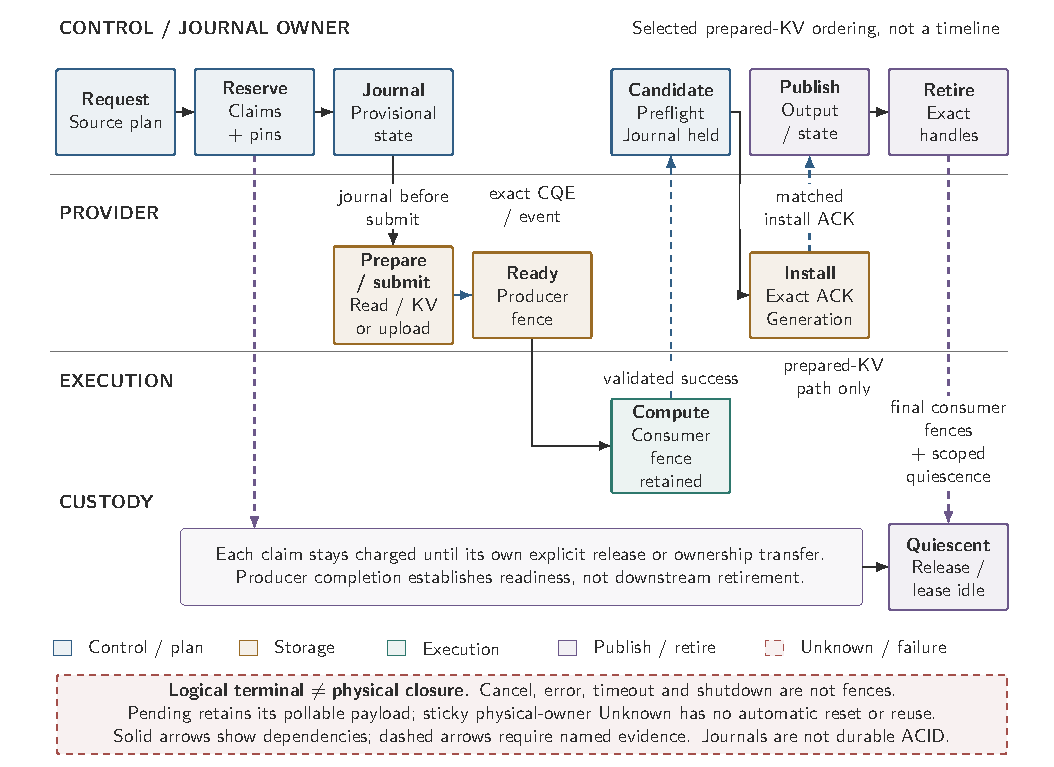
\includegraphics[width=\linewidth]{figures/transaction-lifecycle.pdf}
\caption{Conceptual successful lifecycle for the selected prepared-KV owner,
not a measured overlap timeline. Named lanes and swatches retain blue
control/validation, ochre materialization, teal execution, violet
publication/custody, and brick Unknown/failure roles. The provisional journal
precedes backend preparation even if submission fails without a handle.
Candidate readiness validates existing evidence; exact generation-matched
install ACKs precede logical publication on this path. Producer readiness is
not consumer retirement. Final relevant fences and scoped quiescence precede
custody return, with explicit release/transfer still required. Cancellation
cannot reverse irreversible ending. Neither durable ACID, universal registry
integration, nor general cross-rank atomicity follows.}
\label{fig:transaction-lifecycle}
\end{figure}

\paragraph{Unknown and collective scope.}
Provider Unknown retains native tickets, allocations, claims, and cleanup
intent, and may poison slot layers, devices, or executors. A matching registry
completion can close a named obligation without resetting independent poison.
There is no general in-place reset/replay or device-reset recovery claim.
Prepared-KV coordination is a narrow state lifecycle, not arbitrary distributed
atomic publication. Current collective exchanges have separate host-payload
bounds; Mixed device participation defaults to disabled/host. A typed device
permit is not evidence of a default GPU reduction or cross-rank fence. For the
vLLM supplement, Socket-plugin initialization is not proof that local GPU
payload used Socket: the scoped logs record \texttt{NCCL\_P2P\_DISABLE=1}
and local channels \texttt{via SHM/direct/direct}. No NCCL capability or
transport conclusion is generalized beyond the recorded profile.

\paragraph{What must be traced.}
A full path audit names each progress owner, queue/limit, dependencies,
submission behavior, completion evidence, blocking calls, locks, and
synchronization from request admission through storage, expansion, transfer,
execution, publication, retirement, cancellation, and shutdown. Include
model-specific and host-KV bypasses. A worker wrapping a blocking call is not
proof of event-driven progress or hardware overlap. Current BF16/numeric and
Mixed TP profiles have distinct shard/cache/expansion policies; actual storage
integration and residency require profile-specific evidence. Shared/unified
physical pools and other modalities remain design scope, not evaluated
support. Rust ownership assists local reasoning but does not discharge
asynchronous physical references owned by providers.

\section{Evaluation: Setup and Four Research Questions}
\label{sec:evaluation}
\label{sec:core-rqs}

We report an exploratory TP1 logical-demand observation and separate TP2
numerical and resident-serving records. We do not combine profiles to create
a quality, capacity, or performance result. E0 (RQ1), E3 (RQ2), the safe
blocking/async part of E1/E4 (RQ3), and integrated E5 (RQ4) retain their
historical experiment identifiers. Broad serving sweeps (E2), further
ablations (E4), and protocol overhead (E6) remain secondary evidence plans.

\subsection{Setup, controls, and evidence units}
\label{sec:eval-setup}
The TP1 middle experiment uses Qwen3.5-35B-A3B-FP8, one CUDA owner
(PP1/TP1/EP1, thread), the resident engine, lazy experts, resident KV,
context 128, batch-token limit 8, active-sequence limit 2, and prefill chunks
of 8. Its Mixed arithmetic uses BF16 activation/KV/convolution with F32
accumulation/SSM; the FP8 checkpoint is not a complete arithmetic contract.
The sealed binary is \texttt{36e6aaa5\ldots70a58c}. Table~\ref{tab:tp1-config}
reports configured limits, not physical partitions.

\begin{table}[tbp]
\centering
\small
\begin{tabularx}{\linewidth}{@{}lX@{}}
\toprule
Configured field & Value / scope \\
\midrule
Device admission / workspace & 7,168 / 2,048 MiB; not a measured total working-set cap \\
Expert cache / scratch & 64 entries; $b_{\mathrm{cache}}=335{,}544{,}320$ bytes (320 MiB, shared cache-accounting ceiling for resident, pending, and scratch); separate $b_{\mathrm{scratch}}=8$ MiB \\
KV / maximum tensor & 16 / 1,024 MiB; distinct covered limits \\
Host expert retention & Zero; not zero OS page-cache residency \\
Request queue / inflight & 2 / 2; actual workload concurrency 1 \\
Physical host limit / caches & Host cap unknown; page cache uncontrolled, not storage-cold \\
Logging / generation & \texttt{ferrule\_performance=DEBUG}; temperature 0, seed 1 \\
\bottomrule
\end{tabularx}
\caption{TP1 middle configuration. Values from the frozen case manifest;
heterogeneous or overlapping limits cannot be added as physical memory.}
\label{tab:tp1-config}
\end{table}

Here $b_{\mathrm{cache}}$ is a configured cache-accounting ceiling, not a
physical-memory bound. The plot field \texttt{cache.peak\_bytes} (raw receipt
key \texttt{expert\_owner\_peak\_bytes}) reports the lifetime high-water of
cache-charged bytes: resident plus pending-upload reservations plus scratch. That charged peak is governed by
the 320 MiB configured cache ceiling. It is not a complete physical-owner
memory peak or an independent measurement of allocator retirement; a total
physical-owner ceiling remains unknown. The configured cache flag includes
scratch according to the sealed startup plan, while $b_{\mathrm{scratch}}$
is a separate component limit. A shared cache byte ceiling constrains resident, pending,
and scratch charge; it is not a separate resident-only budget.

\paragraph{Attempt and request accounting.}
The initial CPU-prepared entry was unexecuted after its final validation was
canceled. Authorized attempt \texttt{-01} then failed before server launch
with a harness \texttt{AttributeError} for missing \texttt{subprocess.DEVNULL}:
planned 4, dispatched 0, not-run 4. No model/OOM, read, request-latency, or
quality result was obtained. Authenticated drain/post-idle checks passed,
while physical I/O and the resource contract remained unknown and GPU
quiescence unverified. This attempt is retained, not pooled with \texttt{-02}.

Attempt \texttt{-02} dispatched four serialized requests: Hello2 and the QA,
arithmetic, and Chinese canaries. All four reached successful HTTP termination;
failed and not-run counts were zero. They returned 26 usage output tokens in
30 decoder invocations. Hello2 has no reference and passed HTTP/usage only.
The other three passed their frozen visible-text/eight-output-token-usage
checks (3/3); QA is one canary, not an extended QA workload. Generated IDs,
logits, routes, and full current-model quality were not observed. This is one
independent DEBUG-instrumented run ($n=1$); observer/logging overhead was not
measured. Its request timings are exploration, not a fast baseline or
steady-state comparison.

TTFT is send-to-first-nonempty SSE content and E2E is send-to-EOF. SSE events
and usage are not exact token timestamps; no exact-token TPOT is reported.
Named request/time/log-byte anchors attribute serialized invocation deltas;
a transaction ID is not a request ID. Memory samples, logical counters,
physical traffic, and owner-ledger occupancy are distinct measurement units.
Freeze snapshot/dirty manifest, binary, model/tokenizer, workload, state
precision, backend, storage, topology, caches, and interval boundaries for
any future comparison. Offered/accepted/completed/failed/rejected/canceled/
timeout counts must remain in the denominator record.

\subsection{RQ1: Capacity and complete quality -- not established}
\label{sec:rq1}
Equations~\ref{eq:physical-capacity} and~\ref{eq:full-residency} define
deduplicated physical capacity and the full-residency test for a declared
complete weight representation;
Equation~\ref{eq:working-set} asks whether the actual streaming working set
fits each domain. The configured limits in Table~\ref{tab:tp1-config} answer
neither question alone. Table~\ref{tab:tp1-memory} reports the available memory proxies without
promoting them to continuously measured $M_d^{\mathrm{peak}}$. The
storage-demand cache figure in RQ2 is a counter/gauge reconciliation, not a
physical-working-set certification.

\begin{table}[tbp]
\centering
\small
\begin{tabularx}{\linewidth}{@{}Xrl@{}}
\toprule
Observable & Reported value & Scope \\
\midrule
Selected GPU0 sampled maximum & 4,125 MiB & 32 GPU samples \\
Server-tree PSS sampled maximum & 7,610.864 MiB & 32 complete host samples \\
Server-tree RSS sampled maximum & 7,613.770 MiB & Same sample population \\
Expert resident entries / bytes & 64 / 201,351,168 & Last invocation gauge \\
Scratch bytes & 8,388,608 & Last invocation gauge \\
Cache charged-byte high-water & 219,754,496 & Lifetime accounting gauge \\
Pending-upload / quarantine bytes & 0 / 0 & Invocation gauges only \\
\bottomrule
\end{tabularx}
\caption{TP1 \texttt{-02} sampled memory and cache-accounting gauges.
Sampled memory maxima are independent, not additive or certified physical
peaks. Cache charged-byte high-water covers resident, pending, and scratch;
its ceiling is 320 MiB, not a physical-owner bound or final ledger proof.
GPU values are selected-device aggregate telemetry, not process attribution.}
\label{tab:tp1-memory}
\end{table}

Host capacity, attributable page-cache residency, continuous peaks, and
process-owned GPU occupancy remain unknown. The OS cache was uncontrolled;
zero host expert retention does not imply zero file residency. Complete
compact weights plus scales/metadata have not been ruled out as a feasible
resident alternative. Nor do four successful HTTP responses constitute the
independent complete-output quality gate. Therefore RQ1 is open: neither
quality-qualified configured-budget feasibility nor inference beyond physical
memory/storage necessity is established by this TP1 record.

\paragraph{Later current-quality gate (2026-10-14).}
The current StorageMiddle64 full40 gate stopped before inference at
\texttt{cuInit}, with \texttt{CUDA\_ERROR\_NOT\_INITIALIZED (3)}: zero
observed numerical metrics/logits, not a numerical mismatch. Fresh-quality and
cold-owner gates were unissued; no retry occurred. Its receipt is
\path{target/validation/}\allowbreak\path{storage-middle64-current-quality-20261014-01/FINAL.json},
distinct from the earlier \texttt{-01} \texttt{DEVNULL} harness failure.
Owner initialization remains under investigation.

\paragraph{Separate TP2 numerical evidence.}
The \texttt{native-whole-capture-full40-02} comparator reports 2,178 exact
fields for each of Hello and Capital, covering prefill and first decode;
max absolute error, RMSE, and field failures are zero, with matching greedy
IDs. This is a separate full-boundary receipt from the six-row selection
below. These are bounded captured/comparator fields, including oracle-only
diagnostics that are not all physically observed device arrays, not a blanket
bitwise claim over the model. The full-boundary audit freezes this scope.
A separate multistep/lifecycle audit records the six cases in
Table~\ref{tab:tp2-numerical}: 33 calls and 35,937 exact comparator metrics.
This table deliberately selects the frozen
\path{experiments/tp2_resident/model-runtime-quality.json} receipt and its
\texttt{cuda-qwen35-mixed-bf16-tp2-local-shards-serial} profile, with test
binary \texttt{a4977b85\ldots e1cc}. A different frozen
\texttt{production-opts-01} acceptance summary, referenced by the optimized
release handoff, reports 37 calls and 40,293 exact metrics across its full40
and six-recipe selection. Its composition/model test binaries and source
snapshot differ. That summary is not substituted for the six rows here:
33/35,937 is the selected denominator for this table only, not a total of all
TP2 validation. Neither count covers the later current-quality gate above.
The frozen greedy4-02 closure records supervisor/drain/release PASS; the older
greedy4-01 supervisor failure remains a failure. These authenticated test
binaries are not public serving binaries. No serving HTTP logits were
observed, and this writing pass did not rerun payload comparisons.

\begin{table}[tbp]
\centering
\small
\begin{tabular}{@{}lrr@{}}
\toprule
TP2 test record & Calls & Comparator metrics \\
\midrule
greedy4-02 & 10 & 10,890 \\
fork2-03 & 6 & 6,534 \\
canary2-01 & 5 & 5,445 \\
recreate1-01 & 4 & 4,356 \\
cold-owner1-01 & 4 & 4,356 \\
cold-owner1-02 & 4 & 4,356 \\
\midrule
Total & 33 & 35,937 \\
\bottomrule
\end{tabular}
\caption[Separate TP2 test-binary numerical/lifecycle evidence]{Separate TP2 Mixed test-binary numerical/lifecycle evidence from
\path{experiments/tp2_resident/model-runtime-quality.json}. Exactness applies
to the frozen comparator metrics, not TP1, vLLM arithmetic, all workloads,
or the current working tree.}
\label{tab:tp2-numerical}
\end{table}

The local frozen F32 process-EP8 full-model pass also remains scoped to its
profile/snapshot, not a thread result or a capacity result. The independent
single-GPU W8A16 strict oracle gate failed on logits, ordered routes, and
internal states; argmax agreement does not reverse that failure. These
records are kept separate from TP1's three limited canaries and from the
resident timing supplement below. Neither quality nor capacity transfers
between profiles merely because a checkpoint is shared.

\paragraph{Experiment needed to close RQ1 (E0).}
Freeze representation/placement and complete-output tolerances; report each
$B_d$, $W_{\mathrm{full}}(r)$, and compact-residency alternative. Measure
physical working-set components and attribution across startup, requests,
and cleanup, stating sampling coverage. Record full-model prefill/multistep
decode for this text instance, repeated materialization/retirement, physical
request reads, retained claims, swap, and cold/warm caches. Sweep configured
budgets separately from physical capacity and retain failed/stalled points.
Use a correct bounded disk-backed reference and a host-only memory-offload
reference where feasible under the same quality/physical contract. An
infeasible reference is infeasible, not zero time or infinite speedup.

\subsection{RQ2: Request I/O -- logical demand observed, physical I/O unknown}
\label{sec:rq2}
\label{sec:tp1-storage-middle}
For request $q$, the additive invocation observables are
\begin{equation}
\begin{aligned}
 L_q&=\sum_{v\in\mathcal V_q}\Delta_v\mathrm{reader\_bytes},\\
 H_q&=\sum_{v\in\mathcal V_q}\Delta_v\mathrm{facade\_H2D\_bytes},\qquad
 \Delta_q=H_q-L_q.
\end{aligned}
\label{eq:request-io}
\end{equation}
$L_q$ is logical checkpoint-reader demand and $H_q$ is facade transfer
activity. Their difference $\Delta_q$ compares two recorded counter layers; it is neither backing-storage traffic nor a physical bus
measurement. In particular, $L_q,H_q,\Delta_q$ do not imply physical
$P_q^{\mathrm{net}}$ or $P_q^{\mathrm{blk}}$. Table~\ref{tab:tp1-storage-middle}
and Figure~\ref{fig:storage-demand-logical-transfer} apply these sums; gauge
values in Table~\ref{tab:tp1-memory} are not summed.

\begin{table}[tbp]
\centering
\small
\begin{tabularx}{\linewidth}{@{}Xrrrrr@{}}
\toprule
Request & Logical read & Uploads & Evictions & TTFT & E2E \\
 & GiB & experts & experts & s & s \\
\midrule
Hello2 & 2.813 & 960 & 896 & 4.265 & 9.186 \\
QA canary & 10.777 & 3,678 & 3,678 & 8.332 & 18.309 \\
Arithmetic canary & 10.396 & 3,548 & 3,548 & 5.308 & 14.110 \\
Chinese canary & 9.766 & 3,333 & 3,333 & 2.605 & 9.932 \\
\bottomrule
\end{tabularx}
\caption{Four serialized TP1 \texttt{-02} requests. Logical GiB
($1\,\mathrm{GiB}=2^{30}$ bytes) and HTTP timings are rounded to three
decimals; expert counts are exact invocation deltas. Not physical storage,
bus traffic, kernel timing, or comparative performance.}
\label{tab:tp1-storage-middle}
\end{table}

The 30 invocations total 69,114 checkpoint-reader calls and
36,240,064,128 logical bytes, 88,763 facade H2D copies and 36,240,248,688
facade bytes, zero recorded expert hits, 11,519 expert uploads, 11,455
evictions, and 34,557 artifact uploads. Thus the four-request aggregate is
$\Delta=184{,}560$ bytes, or 180.234375 KiB; this small difference is an
application-counter distinction, not evidence of disk traffic. Upload counts
are not observed cache misses or measured I/O credits. These counters show
repeated materialization activity, not the general registry's path integration
or physical NAS/network/block-device reads. Startup reads are outside the sums.

\paperplot{figures/storage-demand-logical-transfer.pdf}
{Paired logical checkpoint-reader and facade H2D byte deltas for four serialized
requests in storage-demand TP1 middle -02. GiB means $2^{30}$ bytes; the right
panel resolves the small H2D-minus-reader differences in KiB ($2^{10}$ bytes).
These are application counters, not physical storage I/O or physical bus
traffic; startup I/O is outside invocation accounting
(Equation~\ref{eq:request-io}).}
{fig:storage-demand-logical-transfer}

For the expert-entry count, let $I_j$ and $E_j$ be the recorded install/upload
and eviction deltas for completed invocation $j$, and let $N_j$ be the entry
gauge at that invocation boundary. The observed-boundary relation is
\begin{equation}
 N_j=N_{j-1}+I_j-E_j,\qquad j=2,\ldots,30.
 \label{eq:entry-reconciliation}
\end{equation}
For the first boundary, $N_0^{\mathrm{implied}}=N_1-I_1+E_1=0$;
this is an implied initial condition, not a measured pre-request gauge. Across
the run, 11,519 uploads minus
11,455 evictions equal the last observed 64 resident entries; all subsequent
observed boundaries have zero balance residual. This is entry-count
reconciliation, not byte conservation, continuous occupancy, or a final
owner-ledger proof.

Figures~\ref{fig:storage-demand-cache-reconciliation} and
\ref{fig:storage-demand-invocation-timeline} show the aggregate and
per-invocation forms of Equation~\ref{eq:entry-reconciliation}. The timeline
contains 3/9/9/9 invocation boundaries assigned by serialized request/log-byte
anchors, not 30 output-token or elapsed-time samples.

For the cache-gauge subset, define
\begin{equation}
\begin{aligned}
 C_j^{\mathrm{cache}}&=X_j+Q_j+S_j,\\
 C_{\mathrm{peak}}^{\mathrm{cache}}
   &=\max_{u\in\mathcal U_{\mathrm{owner}}}C_u^{\mathrm{cache}}
     \leq b_{\mathrm{cache}}.
\end{aligned}
\label{eq:cache-charge}
\end{equation}
where $X_j$ is resident expert bytes, $Q_j$ pending-upload bytes, and $S_j$
scratch bytes at invocation boundary $j$. Unknown-quarantine bytes $Z_j$ are
an already charged retained subset of $C_j^{\mathrm{cache}}$, not an
additional term. This subset is distinct from general-ledger retained $T_a$. These are cache-owner counter semantics, not evidence that
all physical allocations or grants were observed. This is an observed cache
subset, not $M_d(t)$ and not the complete $F_a+R_a+I_a+L_a+T_a$ ledger. At the
last
invocation, the recorded values are $X_j=201{,}351{,}168$ bytes,
$Q_j=0$, and $S_j=8{,}388{,}608$ bytes; the reported $Z_j$ is zero.
Equation~\ref{eq:cache-charge} adds compatible gauges at that one boundary,
not maxima or observations across time. Figure~\ref{fig:storage-demand-cache-reconciliation}
keeps the plotted gauges separate. $\mathcal U_{\mathrm{owner}}$ denotes
cache charged-state update points over the owner's lifetime, not just the 30
invocation samples. The recorded \texttt{cache.peak\_bytes} is
$C_{\mathrm{peak}}^{\mathrm{cache}}=219{,}754{,}496$ bytes, an accounting
high-water governed by \texttt{ExpertCacheLimits.max\_bytes}, namely
$b_{\mathrm{cache}}=335{,}544{,}320$ bytes. This is the
cache admission/charging contract, not independent verification of every
allocation or the general credit partition. Neither the peak nor
$b_{\mathrm{scratch}}$ certifies total physical-owner memory, continuous
$M_d(t)$, or shutdown custody closure. Unknown quarantine remains an already
charged subset and does not add another copy of the charge.

\paperplot{figures/storage-demand-cache-reconciliation.pdf}
{TP1 middle -02 entry reconciliation and cache-accounting gauges.
Uploads minus evictions ($11{,}519-11{,}455=64$) match the last observed
entries; initial zero is implied, not measured, and subsequent boundaries
reconcile. Recorded \texttt{cache.peak\_bytes}, 209.574 MiB, is the
resident-plus-pending-plus-scratch high-water, bounded by
\texttt{ExpertCacheLimits.max\_bytes} = 320 MiB, not a physical-owner bound.
Total physical-owner peak/ceiling are unobserved; no contradiction is implied.
Invocation gauges and lifetime high-waters are not accumulated or a final
ledger proof (Equations~\ref{eq:entry-reconciliation} and~\ref{eq:cache-charge}).}
{fig:storage-demand-cache-reconciliation}

\paperplot{figures/storage-demand-invocation-timeline.pdf}
{Per-invocation expert upload/eviction deltas and resident-entry observations
for the 30 completed invocations in storage-demand TP1 middle -02. Serialized
request/log-byte anchors assign the 3/9/9/9 invocations to requests. The x-axis
is log-order invocation ordinal, not elapsed time, output-token index, or
transaction-as-request ID. Entry occupancy is observed only at invocation
completion, not continuously; uploads are not inferred cache misses
(Equation~\ref{eq:entry-reconciliation}).}
{fig:storage-demand-invocation-timeline}

Startup was 18.497 s. Four separate HTTP windows sum to 51.538 s, excluding
startup and inter-request owner overhead; supervisor wall time was 75.874 s.
The origins in Figure~\ref{fig:storage-demand-timing} are explicitly
\begin{equation}
\begin{aligned}
 T_{\mathrm{start}}&=t_{\mathrm{ready}}-t_{\mathrm{launch}},\\
 T_q^{\mathrm{first}}&=t_q^{\mathrm{first\ content}}-t_q^{\mathrm{send}},\qquad
 T_q^{\mathrm{end}}=t_q^{\mathrm{EOF}}-t_q^{\mathrm{send}}.
\end{aligned}
\label{eq:timing-origins}
\end{equation}
These are distinct denominators. Startup has a launch origin; each request
bar has its own HTTP send origin, not one cumulative timeline. It therefore
does not imply an end-to-end throughput
rate or an I/O bottleneck share. $P_q^{\mathrm{net}}$ and
$P_q^{\mathrm{blk}}$ remain unknown. Logical reader/syscall bytes can be
served by cache; facade transfers are not physical bus measurements.

\paperplot{figures/storage-demand-timing.pdf}
{Launch-to-ready startup and per-request HTTP TTFT/E2E in the single successful
DEBUG-instrumented storage-demand TP1 middle -02 run ($n=1$). TTFT is send to
first nonempty SSE content; E2E is send to EOF. Startup has a different origin
and is not part of the request bars. Instrumentation overhead is unmeasured;
there are no statistics, confidence intervals, kernel timings, or comparative
speedups (Equation~\ref{eq:timing-origins}).}
{fig:storage-demand-timing}

To close RQ2 (E3), align application, process, mount/network, and backing-block
observations to the same requests and declared cache policy, with foreign
traffic and attribution limits. Distinguish startup from requests, runtime
cache from OS/shared file cache and storage-server cache, and physical disk
reads from memory migration. A warm request with no backing read is valid but
not evidence of request-time disk access. Swap traffic must be disclosed,
not silently counted as the intended storage path.

\subsection{RQ3: Safe scheduling -- reference not implemented}
\label{sec:rq3}
The same-contract safe-blocking reference on the actual TP1 path is
\textbf{not implemented}. Neither \texttt{-02}'s HTTP latencies nor the
resident TP2/vLLM supplement compare blocking and asynchronous scheduling.
There is no measured physical-overlap, event-driven-progress, or causal
scheduling benefit in the current evidence.

The E1/E4 experiment must first audit the actual path specified in
Section~\ref{sec:implementation}, including bypasses. Implement a correct
bounded blocking reference and serialize selected stages only while keeping
weights, arithmetic, quality, caches, ledgers, sharing/custody, and publication
rules fixed. Unsafe buffer reuse or unbounded queues are not simplification
controls. Record submission/completion and true provider/accelerator intervals,
operation/generation identities, dependency readiness, queue/claim occupancy,
blocked workers, locks, and synchronization. Correlate clocks and report
uncertainty before intersecting storage/transfer/compute intervals. Host
enqueue intervals alone cannot prove physical overlap. Include exhausted
budgets, stalled owners, and full queues to expose cyclic waits/starvation
under the stated conditional-liveness assumptions.

\subsection{RQ4: Custody and failure -- final resource contract unknown}
\label{sec:rq4}
For TP1 \texttt{-02}, authenticated descendant drain reached \texttt{ECHILD};
wrapper post-idle and independent all-eight-GPU observational idle checks
passed. Nevertheless \texttt{resource\_contract\_complete=unknown} and the
supervisor raw \texttt{gpu\_quiescence=unverified} remain unchanged. Invocation
pending-upload/quarantine gauges of zero are not a final owner ledger.
Process drain and idle telemetry establish neither device fences nor source
completion nor the partition in Equation~\ref{eq:credit-conservation}.

Algorithm~\ref{alg:terminal-custody} therefore specifies the required
behavior, not the measured closure of this run. E5 must inject delayed/stale
completion, stage-wise cancellation, primary-plus-cleanup failure, owner loss,
and lost ACKs on the integrated path. Track exact publication/reuse, original
versus repeated submissions, ownership transfers, retained $T_a$, named
completion proofs, drain, and post-failure service. Reconcile grants and
allocations before and after proven quiescence; distinguish deterministic
protocol injection from real hardware failure. Unknown should remain charged
and unusable without fabricated rollback or recovery. A failed/stalled
provider also tests liveness assumptions, not just safety. Integrated fault
conservation, eventual reclamation, and final TP1 custody closure remain open.

\subsection{Supplement: resident observations, not an RQ1--RQ4 substitute}
\label{sec:resident-supplement}
\paragraph{Supplementary resident TP2 observations.}
The frozen route-batch crossblocks record contains two independent blocks
in F1--V1 and V2--F2 order, with four fresh server owners. Each slot excludes
three QA8 requests and then measures five requests, each with five input
and eight output tokens: 40 output tokens per measurement window.
Table~\ref{tab:resident-crossblocks} transcribes these existing observations;
no new measurement is introduced here.

\begin{table}[t]
\centering
\small
\begin{tabular}{@{}lrrrrrr@{}}
\toprule
Slot & Output & TTFT & E2E & Startup & GPU & PSS \\
 & tok/s & ms & ms & s & GiB/card & GiB \\
\midrule
F1 & 14.317 & 176.248 & 523.399 & 349.585 & 21.04 & 61.05 \\
V1 & 10.376 & 132.676 & 694.228 & 66.239 & 19.28 & 7.71 \\
V2 & 10.330 & 134.651 & 699.213 & 62.814 & 19.28 & 7.32 \\
F2 & 14.804 & 171.333 & 515.106 & 366.133 & 21.04 & 60.14 \\
\bottomrule
\end{tabular}
\caption{Descriptive resident TP2 crossblocks ($n=2$). TTFT and E2E are
request means; GPU and server-tree PSS are sampled peaks, not exact peaks
or per-owner GPU attribution. F denotes Ferrule; V denotes vLLM.}
\label{tab:resident-crossblocks}
\end{table}

Ferrule has a higher output rate and lower mean E2E in both short windows;
vLLM has lower mean TTFT, shorter startup, and lower sampled GPU and host
PSS. The descriptive F/V rate ratios are 1.380 and 1.433, not statistical or
causal speedups. The record uses a pinned checkpoint and tokenizer with
TP2, context 128, batch 8, sequence limit 2, and concurrency 1. Ferrule's
FP8-checkpoint/BF16 activation, KV and convolution/F32 SSM path uses
HF-eager-qualified GemmEx/routing, whereas vLLM uses BF16/FP8 Marlin.
These are not bit-exact or arithmetic-equivalent implementations, and the
record retains \texttt{fairmatch=false} and \texttt{exact\_speedup=null}.
Ferrule's 22 GiB/device admission budget, including a 4 GiB workspace with
a 3 GiB arena, is not identical to vLLM's utilization setting of 0.8.
The common sampled 22 GiB ceiling is not a hard physical partition or a
matched total GPU/host working-set budget.

The measured vLLM deployment is \texttt{0.28.0+cu129}, with
\texttt{Torch 2.13.0+cu129}; its installed identities are frozen under
\path{target/vendor/vllm028-py312}, not inferred from a 0.18 source checkout.
Visible-text/usage canaries and Ferrule's separate scoped oracle records do
not establish cross-engine internal-state parity or universal task quality.
These resident windows neither demonstrate request-time physical disk reads
nor establish host-memory insufficiency, storage necessity, or E0 acceptance.
The immutable source record is
\path{papers/arxiv/experiments/tp2_resident/runs/route-batch-vllm-crossblocks-20261012-01/crossblocks-results.md},
with raw metrics in the adjacent \path{crossblocks-results.json} and frozen
identities in \path{sealed-identities.json}. Historical pilots and failed
attempts remain separate records, not pooled repetitions of this configuration.


\paragraph{Supplementary startup-metadata observations.}
The sealed release \texttt{36e6aaa5\ldots70a58c} combines prepared admission
and shared \texttt{Arc<Path>} checkpoint read-plan metadata. Its strict TP2
S1/S2 smoke lifecycles and ordinary F1 completed with source-bound executable
and mapped-library checks. S1/S2 passed visible greedy canary, reuse,
cancellation-policy and post-cancel gates, with authenticated descendant
drain. These are scoped serving checks, not a fresh 14-million-logit numerical
validation or proof of device quiescence from process exit.
Table~\ref{tab:startup-metadata} separates smoke and performance records.

\begin{table}[t]
\centering
\small
\begin{tabularx}{\linewidth}{@{}Xrrr@{}}
\toprule
Record & Startup & Peak tree PSS & Usage rate \\
 & s & GiB & tok/s \\
\midrule
36e6 S1 (smoke) & 222.079 & 42.716 & --- \\
36e6 S2 (smoke) & 139.855 & 44.416 & --- \\
36e6 F1 (ordinary) & 140.052 & 43.573 & 13.899 \\
e674 F1 (historical ordinary) & 351.114 & 60.149 & 14.227 \\
\bottomrule
\end{tabularx}
\caption{Startup and sampled PSS observations. Smoke slots have no QA8
throughput measurement. The historical ordinary row is context, not a
paired before/after control.}
\label{tab:startup-metadata}
\end{table}

F1 excludes three QA8 requests and measures five, each with five input and
eight output tokens: 40 usage output tokens over 2.877869 s. Its request
TTFT mean/p50/p95 are 192.944/187.513/209.700 ms, descriptive summaries of
five requests, not independent-trial confidence intervals. S1, S2, and F1
are not pooled, and the best startup is not treated as a stable constant.
The historical ordinary e674 F1 is a different series from the crossblocks
in Table~\ref{tab:resident-crossblocks}; no fresh BEFORE or de288 control
was run. Page-cache state is uncontrolled, not cold. Startup, sampled PSS,
and output-rate tradeoffs therefore do not identify a causal optimization
effect, live-heap reduction, freed OS memory, or a storage-capacity result.

Five F1 proc snapshots, in first-identification, ready, post-warmup,
post-measurement, and post-exit order, cost
0.643/623.616/725.908/625.392/0.085 ms to read and validate. Their recorded
bounds all lie outside the measured window; receipt writes are also outside,
but persistence cost was not separately measured. This excludes those reads
from the stated denominator, not observer overhead from the system. On the
recorded Linux 4.19 deployment, \texttt{Pss\_Anon}/\texttt{Pss\_File} are
unavailable; the post-exit snapshot is unavailable, not zero memory.

The source-relation proof records unchanged model mathematics, backend/native
kernels, and runtime, while checkpoint representation differs. CPU IO-byte,
ordering, and source-check tests support compatibility, not fresh GPU numerical
acceptance; full-checkpoint payload hashing was not performed. Thus metadata
representation and source-bound plans have implementation evidence, while the
physical request-time storage frontier remains unvalidated.

The local reproducibility entry \path{REPORT.md} is in:
\begin{quote}
\small\path{target/validation/startup-metadata-owner-20261013-01}
\end{quote}
Its \path{RESULTS.json} supplies the full binary hash and raw-pin manifest;
\path{executed-source-pins.json} identifies executed Python/config revisions.
The F1 raw HTTP and \path{proc-timeline.json} are under the repository's
paper experiment runs directory, at:
\begin{quote}
\small
\path{papers/arxiv/experiments/tp2_resident/runs}/\\
\path{startup-metadata-info-after-20261013-01}/\\
\path{runs/F1/session}
\end{quote}
Historical ordinary raw pins are in \path{routebatch-performance.json},
under the sibling directory \path{route-batch-info-after-20261012-01}.
These working-directory artifacts still require portable archival; they have
not been moved or repackaged for publication.


\subsection{Evidence gates and reproducibility}
\begin{table}[tbp]
\centering
\small
\begin{tabularx}{\linewidth}{@{}l>{\raggedright\arraybackslash}X>{\raggedright\arraybackslash}X@{}}
\toprule
Question & Available observation & Gate still open \\
\midrule
RQ1 & TP1 HTTP/canaries and sampled device/tree memory & Complete numerical quality, physical capacities/working-set peaks, compact-residency alternative \\
RQ2 & 36,240,064,128 logical bytes; $L/H$ transfer difference and entry/cache plots & Request physical network/block I/O and controlled caches \\
RQ3 & Algorithms and path-audit requirements & Safe-blocking reference not implemented; no physical overlap trace \\
RQ4 & Authenticated drain and observational idle & Resource contract unknown; device quiescence unverified; integrated fault/ledger evidence \\
TP2 supplement & Separate numerical tests; two resident crossblocks & No TP1 transfer, arithmetic parity, fair speedup, or capacity proof \\
\bottomrule
\end{tabularx}
\caption{Observable-to-claim map. An open gate is not filled by a result from
another representation, binary, topology, or workload.}
\label{tab:evidence}
\end{table}

The fixed TP1 reports are relative to \path{papers/arxiv}, under
\path{experiments/storage_demand/runs/}:
\begin{quote}
\small
\path{storage-demand-tp1-middle-20261013-01/}\allowbreak\path{report.json}\\
\path{storage-demand-tp1-middle-20261013-02/}\allowbreak\path{report.json}
\end{quote}
The latter has adjacent \path{case.json}, \path{server.log},
\path{samples.jsonl}, \path{supervisor.json}, \path{custody.json}, and
\path{post-idle.json}. The independent closeout is under
\path{../../target/validation/}:
\begin{quote}
\small
\path{storage-demand-middle-gpu-20261013-02/}\allowbreak\path{closure.json}
\end{quote}
The deterministic offline receipt analysis is in
\path{experiments/storage_demand/analysis/output/}; it reports source
consistency PASS with 41 bound inputs, 39 consumed receipt pins, and zero
divergences. That is a receipt-consistency check, not a new GPU or numerical
acceptance result. The TP2 numerical sources are
\path{experiments/tp2_resident/full-boundary-audit.json} and
\path{experiments/tp2_resident/model-runtime-quality.json}. The separate
37-call selection and its handoff are under \path{../../target/validation/}:
\begin{quote}
\small
\path{tp2-mixed-production-opts-01/}\allowbreak\path{acceptance-summary.json}\\
\path{tp2-mixed-optimized-release-20261009/}\allowbreak\path{handoff.json}
\end{quote}
All paths in this paragraph are relative to \path{papers/arxiv}.

Publication requires portable frozen artifacts: source plus dirty-state
manifest, binary, model, and input-processing identities, commands and environment,
raw results, traces/clock-correlation method, retained failures, and
deterministic plot/table generation. Local ignored \path{target/} files and
private transcripts are not public artifacts. Do not silently omit failed
trials. Before confirmatory collection, freeze trial/block units, repetition
counts, order, stopping rules, contrasts, and interval methods. Windows in one
server are not independent repetitions. The historical minimum of five
independent paired performance blocks applies if performance is promoted to
a primary claim; it neither specifies the core RQ repetition counts nor
guarantees power. No statistical victory or universal quality threshold is
inferred from these exploratory records.

\section{Related Work}
\label{sec:related}

\paragraph{Storage-backed inference and memory hierarchies.}
FlexGen~\cite{sheng2023flexgen} distributes tensors across GPU, CPU, and disk
and optimizes throughput-oriented schedules with compression and
attention-cache management. DeepSpeed-Inference~\cite{aminabadi2022deepspeed}
also provides heterogeneous inference using CPU and NVMe capacity;
ZeRO-Inference~\cite{deepspeed2022zeroinference} describes weight hosting,
layer streaming, prefetch, and release in an official technical web page.
These are direct precedents for inference beyond device residency.
ZeRO-Infinity~\cite{rajbhandari2021zeroinfinity} establishes a related
GPU/CPU/NVMe hierarchy for training, whose optimizer-state and training
results do not directly characterize inference. At the storage-access level,
LLM in a flash~\cite{alizadeh2024llmflash} uses windowing and row-column
bundling to reduce flash weight reads and enlarge useful transfers when a
model exceeds DRAM. These works motivate managing both placement and access
patterns; \system{} focuses on the contract connecting each materialization
stage to source identity, resource claims, completion evidence, and reuse.

\paragraph{Heterogeneous execution and representation.}
PowerInfer~\cite{song2023powerinfer} exploits activation locality by executing
hot neurons on a GPU and cold neurons on a CPU. This differs from
PowerInfer-2~\cite{xue2024powerinfer2}, whose cited smartphone version uses
neuron clusters, segmented caching, and an I/O/computation pipeline beyond
resident capacity. CPU execution, storage traffic, and device-cache residency
are therefore separate comparison dimensions. Weight representation is
another independent axis: AWQ~\cite{lin2024awq} uses activation-aware scaling
to protect salient weights during low-bit quantization. Representation and
materialization scheduling can be considered separately, but equal bit widths
do not establish equal algorithms, quality, or execution costs. This citation
does not imply that \system{} implements or evaluates AWQ.

\paragraph{Expert caching, prediction, and execution location.}
Direct MoE offload systems already exploit selective expert demand.
MoE-Infinity~\cite{xue2024moeinfinity} uses activation traces to guide GPU
expert-cache replacement and prefetch for host-memory-backed inference on
personal machines. Eliseev and Mazur~\cite{eliseev2023fastmoeoffloading}
combine an LRU expert cache with speculative loading from earlier hidden
states and mixed quantization. Their speculative prefetch does not itself
change routing: a prediction miss still requires the demanded expert;
quantization has a separate numerical-quality boundary.
Fiddler~\cite{kamahori2025fiddler} instead coordinates moving expert weights
to the GPU with moving activations to CPU experts. Its execution-location
choice is not equivalent to a cache policy that always executes demanded
experts on the GPU. These mechanisms concern different combinations of cache
reuse, transfer avoidance, and heterogeneous computation, not one common
storage or execution path.

\paragraph{Routing and precision changes for expert offload.}
Pre-gated MoE~\cite{hwang2024pregatedmoe} changes gating so that one block
selects experts for the next, enabling migration to overlap current expert
computation. Its pre-gate is trained during fine-tuning while retaining
pretrained parameters; this is a model change rather than speculative
prefetch applied to an unmodified checkpoint.
HOBBIT~\cite{tang2024hobbit} dynamically loads lower-precision versions of
less-critical experts on cache misses, together with adaptive prefetch and
multidimensional caching. Its loading policy thus includes a quality--latency
tradeoff. \system{} instead studies read scheduling and upload grouping with
fixed selected-expert order and arithmetic. That distinction does not establish
superior performance or rule out complementary caching policies.

\paragraph{Demand-loaded expert caches in serving engines.}
The inspected SGLang source includes a specialized expert-pack loader and
runtime cache~\cite{sglang2026expertpack}. Cache misses issue storage reads into
staging slots, followed by event-gated host-to-device copies; preparation of
the packed representation does not eliminate those runtime reads. The loader
and argument checks restrict this path to DeepSeek-V4 Flash and text-only
Kimi-K3, require unit tensor, data, and expert parallelism, and disable CUDA
graphs and shared-expert fusion. These are boundaries of the inspected path,
not claims about every SGLang configuration or future version. We neither ran
this path nor established its release inclusion, numerical qualification, or
relative performance. Its source demonstrates that storage-backed expert
loading is not unique to \system{}; equivalent failure-custody guarantees
have not been exhaustively audited in either direction.

\paragraph{KV allocation, selection, and prefix reuse.}
KV state is a different object from checkpoint weights.
vLLM uses PagedAttention~\cite{kwon2023pagedattention} for block-based KV
allocation and sharing, and its paper includes CPU KV swapping for preempted
requests. The separately inspected CPU-weight-offload paths use host-resident
weights, including unified virtual addressing; these should not be equated
with disk-backed weight materialization. SGLang uses a radix tree for KV
prefix reuse across calls~\cite{zheng2024sglang}; that paper is distinct from
the expert-pack source snapshot above.
Pensieve~\cite{yu2025pensieve} retains conversation state across requests in
a GPU/CPU cache to avoid repeated history processing.
InfiniGen~\cite{lee2024infinigen} instead predicts important tokens and
prefetches selected KV from host memory. Importance-based approximate
selection must be distinguished from retaining complete state: its quality
conditions are not those of exact capacity management.

\paragraph{KV storage and transport.}
Mooncake~\cite{qin2025mooncake} builds a cluster-wide KV-centric serving
architecture using CPU, DRAM, SSD, and network resources, establishing an
explicit storage-backed KV precedent. CacheGen~\cite{liu2024cachegen}
compresses and streams KV with bandwidth-adaptive compression, addressing
network loading and its quality tradeoff rather than only local placement.
D{\'e}j{\`a}Vu~\cite{strati2024dejavu} provides KV streaming for prompt/token
separation, microbatch swapping, and state replication for recovery.
These systems show why reuse scope, storage tier, transfer path, and numerical
semantics must be stated separately. KV transport and replication can support
a serving architecture without being the same mechanism as checkpoint-weight
materialization or establishing its resource-lifetime guarantees.

\paragraph{Request and phase scheduling.}
Orca~\cite{yu2022orca} schedules at generation-iteration boundaries with
selective batching. Sarathi-Serve~\cite{agrawal2024sarathiserve} combines
chunked prefill and stall-free scheduling to manage the throughput--latency
tradeoff. Splitwise~\cite{patel2024splitwise} places prompt processing and
token generation on separate machines according to their resource demands;
DistServe~\cite{zhong2024distserve} separates prefill and decoding to optimize
goodput under latency constraints. At a broader placement level,
AlpaServe~\cite{li2023alpaserve} combines model parallelism and statistical
multiplexing for bursty workloads. These works choose when and where requests
or phases execute. \system{} addresses resource admission and completion
within materialization, not a new request-batching or cluster-placement
algorithm; this positioning implies no cross-system performance ordering.

\paragraph{Execution control.}
Salus~\cite{yu2020salus} separates GPU-sharing primitives, including fast
switching and memory sharing, from scheduling policy.
Clockwork~\cite{gujarati2020clockwork} builds predictable serving around
explicit control of execution and resource behavior.
Tutel~\cite{hwang2023tutel} adapts parallelism and pipelined execution to
dynamic MoE workloads. These works concern execution control rather than the
source-bound materialization lifecycle studied here. Their results do not
establish \system{} performance, predictability, or completion guarantees.

\paragraph{Bounded prefetch and staged admission.}
Informed prefetching~\cite{patterson1995informed} uses future-access hints to
coordinate prefetching with cache-buffer allocation. This precedent treats
lookahead as a consumer of finite buffers, not free early I/O.
SEDA~\cite{welsh2001seda} connects event-driven stages with explicit queues
and stage-local resource control. \system{} applies bounded admission to
materialization claims; it does not implement those systems' buffer-allocation
algorithms or adaptive controllers.

\paragraph{Publication and safe reclamation.}
Linearizability~\cite{herlihy1990linearizability} is a correctness condition
for concurrent-object histories, not a resource-reclamation mechanism or a
persistent transaction protocol. Hazard pointers~\cite{michael2004hazard}
distinguish logical removal from safe reclamation after concurrent use ends.
\system{} uses a local publication and completion protocol with owner-held
evidence through retirement. This is neither a linearizability proof nor a
persistent ACID protocol, and the reclamation analogy does not imply a
hazard-pointer implementation or a general device-reclamation theorem.

\paragraph{Measurement and comparison boundaries.}
An asynchronous interface, an independent progress worker, and hardware
overlap are distinct properties. The earlier read-scheduling comparison holds
worker, representation, and resource limits fixed, then changes when one
next-expert read is submitted. The transfer-policy comparison instead holds
the read schedule fixed and changes upload grouping. Client timing measures
the resulting behavior; correlated file-call and kernel intervals separately
measure observed read--compute overlap. Selected-process API counts quantify
observed synchronization calls, not a complete causal decomposition. Neither
a worker, a broad host-range intersection, nor fewer synchronization calls
alone establishes device overlap or faster serving. A fair external comparison
must also match representation, arithmetic, physical memory pools, workload,
and quality criterion. The unmatched resident-system observations preserved
with the artifacts do not satisfy those conditions and support no comparative
speedup or ranking here.

\begin{table}[!htbp]
\centering
\small
\begin{tabularx}{\linewidth}{@{}>{\raggedright\arraybackslash}p{0.20\linewidth}>{\raggedright\arraybackslash}X>{\raggedright\arraybackslash}X@{}}
\toprule
System & Resource focus & Principal mechanism \\
\midrule
FlexGen & GPU, CPU, disk & Tensor placement, batching, compression \\
ZeRO-Inference & CPU or NVMe to GPU & Layer streaming and prefetch \\
PowerInfer & GPU--CPU residency & Hot/cold neuron execution \\
PowerInfer-2 & Smartphone memory/storage & Neuron clusters and I/O pipeline \\
SGLang expert pack & Storage to GPU expert cache & Demand reads, staging, event-gated copies \\
vLLM & Serving KV residency; host-weight offload & PagedAttention; separate resident offload paths \\
\bottomrule
\end{tabularx}
\caption{Mechanism-level positioning from the cited papers and inspected source.
The SGLang entry concerns its specialized expert-pack path, not all adapters.
These are not matched performance measurements.}
\label{tab:prior-work}
\end{table}

\system{} contributes a profile-scoped account of source binding, stage-local
admission, publication, and retirement, together with measurements that keep
logical and physical observations separate. We have not exhaustively audited
the custody or failure semantics of the systems above and do not claim that
they lack equivalent mechanisms. Model-registry entries and architectural
capability are not substitutes for qualified execution: in particular,
\system{} has no tested DeepSeek-V4 serving result. The empirical contribution
is controlled internal comparisons and their explicit resource and completion
scope, not a first-system or state-of-the-art claim.

\section{Limitations}
\label{sec:limitations}

\paragraph{Resource and deployment scope.}
The experiments bound selected logical accounts, not the complete physical
working set. The host limit includes packed and prepared payloads, metadata,
and requested worker stack; OS stack rounding, TLS, allocator overhead,
weak-reference backing, and file-cache residency require additional headroom.
Device samples can miss transient peaks and lack exact process attribution.
The three cache points vary entry and byte limits together, so they neither
isolate a replacement-policy effect nor locate a physical capacity frontier.
The complete compact checkpoint may fit in host memory. Other representations,
long contexts, shared-memory devices, and multimodal workloads remain outside
the evaluated profile.

\paragraph{Statistical and measurement scope.}
The timing study contains five paired blocks of short fixed outputs, not
50 independent repetitions. Shared page and NFS caches can carry state across
fresh servers. The descriptive resampling ranges therefore provide neither
guaranteed coverage nor a significance or power result. Serial-window
goodput excludes startup, gaps, and concurrency. Identical instrumentation
controls one source of bias, but its overhead is unmeasured. The profiling
study observes overlap in two separate requests; it does not identify the
cause of the timing difference. Its target-process checks pass, while
wrapper warnings and an unknown dropped-event count leave global trace
completeness unverified. File-call wall time can include cache service and
preemption, and shared NFS counters do not identify physical backend traffic.

\paragraph{Failure and verification scope.}
The component experiment runs real CUDA operations but injects a software
failure or discards proof after valid fences. It does not exercise a driver
failure, lost hardware event, or full-model uncertain completion. The HTTP
experiment tests a client disconnect followed by a new request, not resumed
execution or recovery from a poisoned owner. Neither experiment establishes
the integrated five-class conservation invariant across a serving request.
Final physical release remains unobserved. Unknown custody can reduce
availability indefinitely; the design supplies no general in-place reset,
durable crash recovery, or arbitrary cross-rank atomic commit.

\paragraph{Reproducibility scope.}
The supplementary materials support offline reconstruction of the public
measurements and their exclusions. They do not independently replay private
process authentication or recover omitted executables, native dependencies,
model payloads, and live mapped-memory contents. Integrity hashes bind retained
inputs but are not external attestations. Earlier rejected or incomplete
studies remain separate rather than becoming successful repetitions.

\section{Conclusion}
\label{sec:conclusion}

Bounded storage-backed inference requires a lifetime contract as well as a
cache policy. \system{} connects source-bound planning and stage-local
admission to exact completion, publication, and custody through retirement.
Its bounded next-expert schedule preserves the blocking control's worker,
budgets, arithmetic, and synchronous consumer proofs. In five paired blocks,
lookahead completes the same checked workload with equal logical reads,
zero wasted read bytes, less host demand waiting, and descriptive reductions
of 8.18\% in end-to-end latency and 11.24\% in time to first content, with
10.91\% higher qualified serial-window goodput. The additional experiments
show bounded completion across three coupled cache budgets, limited measured
read--kernel overlap, safe component abort or retained uncertainty, and
fresh-request recovery after HTTP cancellation. These results support the
mechanism within its measured scope while leaving complete physical
accounting, integrated fault conservation, and final release open.


\bibliographystyle{plain}
\bibliography{references}

\clearpage
\appendix
\section{Qualification History and Stopped CLI Study}
\label{sec:historical-chronology}
Table~\ref{tab:tp1-quality-chronology} separates historical test numerics
from wrapper acceptance, not forecasts for enabled CLI serving. Full40
covers Hello/Capital prefill and one decode; fresh adds bounded history,
feedback, reset and fork. Fixed $\mathrm{atol}=0.00025$,
$\mathrm{rtol}=0.012$ is not bit-exactness or broad task quality.

\begin{table}[H]
\centering
\small
\begin{tabularx}{\linewidth}{@{}lrrX@{}}
\toprule
Record & Metrics & Logit elements & Numerical / wrapper outcome \\
\midrule
Middle quality \texttt{-01} & 0 & 0 & \texttt{cuInit (3)} before inference; fresh/cold unissued \\
Full40 \texttt{-02} & 804 & 1,986,560 & Numerical PASS; original strict post-idle wrapper FAIL \\
Retained fresh \texttt{-03} & 5,427 & 9,187,840 & Numerical PASS; original strict post-idle wrapper FAIL \\
Cold owner \texttt{-04} & 1,809 & 3,228,160 & Numerical and wrapper PASS under stable-idle v2; different source cut \\
Frozen CLI quality \texttt{-01} & 0 & 0 & \texttt{cuInit (3)} before inference; retained fresh unissued \\
\bottomrule
\end{tabularx}
\caption{Later 2026-10-14 TP1 test-gate chronology. Middle quality
\texttt{-01} and frozen CLI quality \texttt{-01} are distinct from the
2026-10-13 prelaunch \texttt{DEVNULL} wrapper failure. Numerical PASS does
not override a rejected wrapper.}
\label{tab:tp1-quality-chronology}
\end{table}

The strict full40/fresh wrappers rejected first post-idle samples of 1\%/6\%
GPU0 utilization (zero MiB, no compute applications); later idle does not
repair them. Cold \texttt{-04} accepts authenticated drain/stable-idle v2
on the 3,533-input \texttt{5662b7d2\ldots} cut, not
\texttt{fbf0c225\ldots}. Its old primary records
\texttt{same\_source\_cut=false} and wrapper rejection; these passes cannot
be pooled. Frozen CLI quality fails at \texttt{cuInit (3)} with zero metrics,
logits and token checks, not numerical mismatch. The later nine-gate
\texttt{033519c} factory PASS changes none of these outcomes. Idle is not
a GPU fence or final resource ledger.

\paragraph{Enabled CLI pilot: permanently stopped.}
\label{sec:paired-startup-failure}
On 2026-10-15, P1-blocking exits before Ready with:
\begin{quote}
\small\ttfamily
invalid runtime request: experimental qwen35-mixed-bf16 serving:\\
prepared source profile changed
\end{quote}
The stopped \texttt{cmd\_serve} called \texttt{mixed\_tp2\_cache\_requirements}
unconditionally; the non-TP2 accessor rejected enabled TP1's prepared-source
payload before CUDA owner startup, not at \texttt{cuInit}. The source-plan
query fix is now committed at \texttt{86c58a0}; this failure is unchanged.
One lifecycle is attempted, zero complete, nine unissued; HTTP issued,
terminal, success, failed and censored counts are all zero, with all
120 requests/50 measured QA slots unissued. All five incomplete pairs stay;
quality metrics, request latencies, goodput, contrasts and intervals are
unobserved/null, not zero. Ready maps, positive reads and the final owner
ledger are unobserved/unknown despite authenticated \texttt{ECHILD}, absent
owners, idle and released/reprobed locks. Shutdown-only shared NFS deltas
are not request-attributable NAS traffic; physical release remains unproved.

Frozen \path{paired-final.json} and \path{closeout.json} are relative to
\path{papers/arxiv}, under:
\begin{quote}
\small
\path{experiments/storage_demand/paired_read_v1/}\\
\path{artifacts-current-20261015-01/}
\end{quote}
No retry/replacement is allowed.
Independent V3 fixes cohort target/deferrals to 1/0, not CLI defaults 4/3.
CPU and hidden-CUDA workspace checks pass for the fix, not new CLI/HTTP
qualification. New same-cut GPU gates and serving binding remain required;
V3 does not resume this study or borrow the old factory PASS.

\end{document}
